\chapter{有限元无网格混合离散方案}

本章针对体积不可压问题建立有限元无网格混合离散方案,调整体积约束比以达到最优约束比。首先介绍了再生核近似无网格法,详细说明了无网格形函数的构造过程,其次介绍实际最优约束比的取值,最后通过典型弹性力学算例验证该最优约束比的正确性。
\section{再生核近似}
为达到最优体积约束比,采用如图\ref{ch_4:fig:meshfree}所示的有限元无网格混合离散方案离散位移和压力节点。
将伽辽金弱形式\eqref{ch_2:eq:weak_mix}中的位移$\boldsymbol{u}$和压力$p$采用不同的离散方式进行近似。
位移$\boldsymbol{u}$仍采用有限元形函数\eqref{ch_2:eq:u_h_mix}进行近似,而压力$p$通过再生核无网格形函数进行近似。
再生核无网格近似将求解域$\Omega$及其边界$\Gamma$由$n_p$个无网格节点离散$\{\boldsymbol x_K\}_{K=1}^{n_p}$。每个无网格节点$\boldsymbol x_K$对应的形函数为$\Psi_K(\boldsymbol{x})$,形函数影响域为$supp(\boldsymbol{x}_K)$。近似的压力$p_h$可表示为:
\begin{equation}
    p_h(\boldsymbol x) = \sum_{K=1}^{n_p} \Psi_K(\boldsymbol x) p_K
\end{equation}
其中$p_K$为与无网格节点$x_K$对应的节点系数。
\begin{figure}[H]
    \centering 
        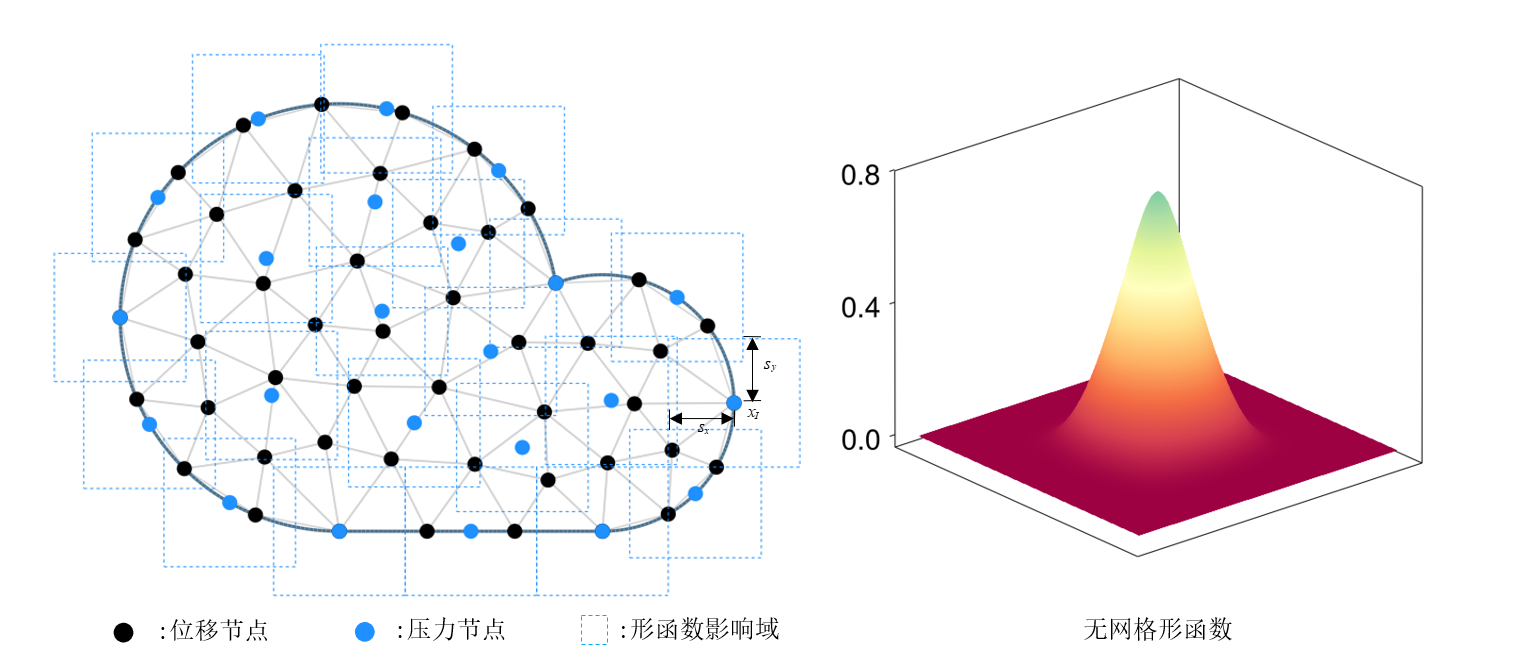
\includegraphics[scale=0.6]{figures/meshfree.png}
        \caption{有限元无网格混合离散示意图}\label{ch_4:fig:meshfree}
\end{figure}

根据再生核近似理论\cite{liu1995},无网格形函数可以假设为如下形式:
\begin{equation}\label{ch_4:eq:rkshape}
    \Psi_K(\boldsymbol x) = \boldsymbol c(\boldsymbol x_K-\boldsymbol x) \boldsymbol p^{[n]}(\boldsymbol x_K-\boldsymbol x) \phi(\boldsymbol x_K - \boldsymbol x)
\end{equation}
其中$\boldsymbol p$为$n$阶基函数向量,其表达式为:
\begin{equation}
    \boldsymbol p^{[n]}(\boldsymbol x) = \{ 1, x, y, x^2, xy, y^2,...,y^n\}^\mathrm{T}
\end{equation}
对于弹性力学问题,无网格基函数一般选择二阶或者三阶多项式基函数,本文选择二阶多项式基函数:
\begin{equation}
    \boldsymbol p(\boldsymbol x) = \{ 1, x, y, x^2, xy, y^2\}^\mathrm{T}
\end{equation}
而$\phi$为核函数,其影响域的大小由影响域尺寸$s$决定,核函数及其影响域的大小共同决定了无网格形函数的局部紧支性和光滑性。在二维情况下,核函数的影响域通常为圆形或者矩形。本文的影响域形状为矩形,矩形影响域的核函数可由下列公式计算得到:
\begin{equation}
    \phi(\boldsymbol x_K-\boldsymbol x) = \phi(r_x) \phi(r_y), \quad r_x = \frac{|x_K - x|}{s_{x}},r_y = \frac{| y_K -  y|}{s_{y}}
\end{equation}
其中, $s_x$ 和 $s_y$ 分别为 $x$ 和 $y$ 方向上的影响域尺寸,若节点均匀布置,一般使两个方向上的影响域大小相等,即$s_x = s_y = s$。
为保证形函数的紧支性和光滑性,$\phi$ 通常取为阶次大于 $n$ 的紧支函数。因此,本文核函数 $\phi(\boldsymbol x_K-\boldsymbol x)$ 取为三次样条函数:
\begin{equation}
    \phi(s) =\frac{1}{3!} \begin{cases}
        (2-2s)^3 - 4(1-2s)^3 & s\le\frac{1}{2} \\
        (2-2s)^3 &\frac{1}{2}<s<1 \\
        0 & s> 1
    \end{cases}
\end{equation}
$\boldsymbol c$为待定系数向量,可以通过满足下列一致性条件确定:
\begin{equation}\label{ch_4:eq:cc1}
    \sum_{I=1}^{n_p}\Psi_K(\boldsymbol x) \boldsymbol p(\boldsymbol x_K) = \boldsymbol p (\boldsymbol x)
\end{equation}
或等效的转换形式:
\begin{equation}\label{ch_4:eq:cc2}
    \sum_{I=1}^{n_p}\Psi_K(\boldsymbol x) \boldsymbol p(\boldsymbol x_K-\boldsymbol x) = \boldsymbol p(\boldsymbol 0)
\end{equation}
将式\eqref{ch_4:eq:rkshape}代入式\eqref{ch_4:eq:cc2}中即可得到待定系数向量$\boldsymbol c$的具体表达式:
\begin{equation}\label{ch_4:eq:correction}
    \boldsymbol c(\boldsymbol x_K-\boldsymbol x) = \boldsymbol A^{-1}(\boldsymbol x_K-\boldsymbol x)\boldsymbol p(\boldsymbol 0)
\end{equation}
式中$\boldsymbol A$为矩量矩阵:
\begin{equation}
    \boldsymbol A(\boldsymbol x_K-\boldsymbol x) = \sum_{I=1}^{n_p}\boldsymbol p(\boldsymbol x_K-\boldsymbol x) \boldsymbol p^{\mathrm{T}}(\boldsymbol x_K-\boldsymbol x)\phi(\boldsymbol x_K-\boldsymbol x)
\end{equation}

将式\eqref{ch_4:eq:correction}代入式\eqref{ch_4:eq:rkshape}可得最终的再生核无网格形函数表达式:
\begin{equation}\label{ch_4:eq:mfshapefunction}
    \Psi_K(\boldsymbol x) = \boldsymbol p^{\mathrm{T}}(\boldsymbol 0) \boldsymbol A^{-1}(\boldsymbol x_K-\boldsymbol x)p(\boldsymbol x_K-\boldsymbol x)\phi(\boldsymbol x_K-\boldsymbol x)
\end{equation}

\section{数值算例}
\subsection{悬臂梁问题}

首先考虑经典弹性力学二维悬臂梁问题,如图\ref{ch_4:fig:cantilever}所示,悬臂梁的长和宽分别为$L=48$,$D=12$,同时悬臂梁的左端为固定支座,
右端沿着$y$轴正方向施加外部荷载$P=1000$。悬臂梁的材料系数为杨氏模量$E=3\times10^6$、泊松比$\nu=0.5-10^{-8}$。
\begin{figure}[!h]
    \centering 
        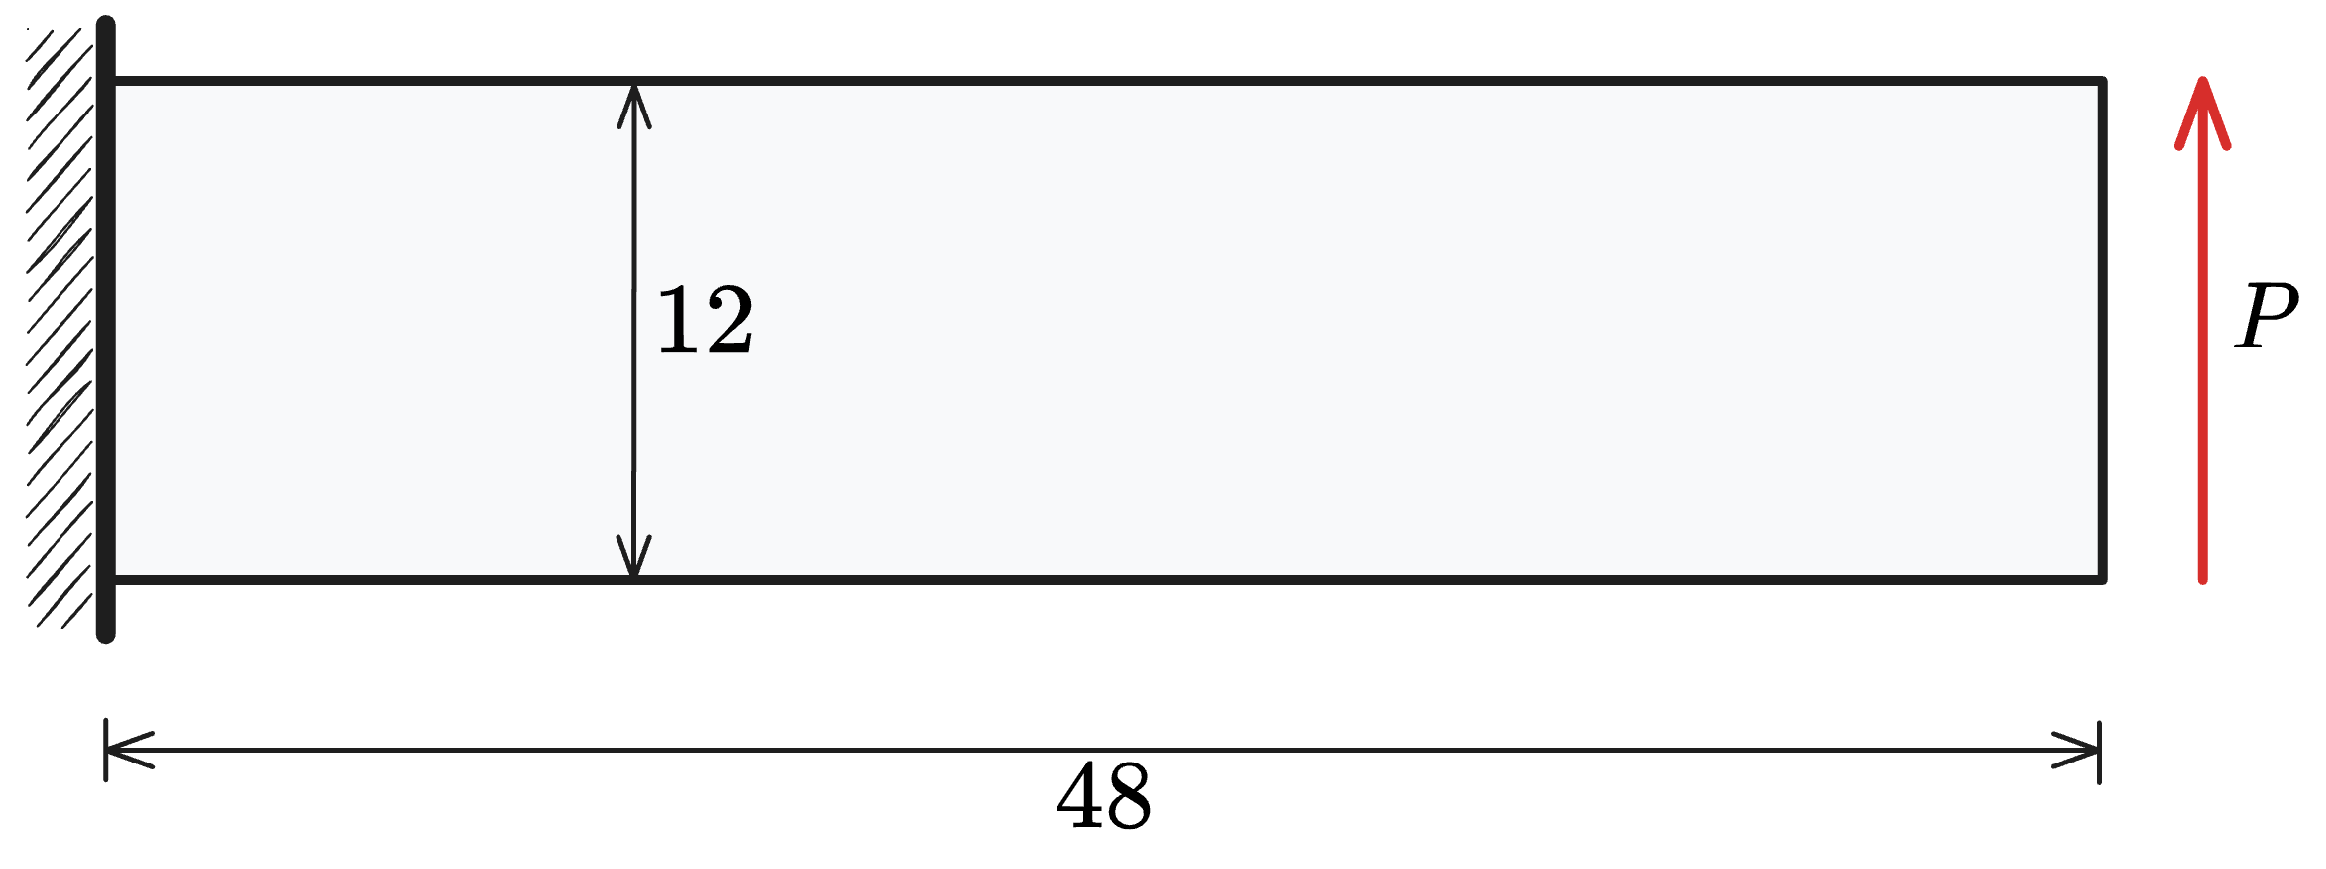
\includegraphics[scale=0.5]{figures/ch_4/cantilever.png}
        \caption{悬臂梁问题模型}\label{ch_4:fig:cantilever}
\end{figure}

根据圣维南原理和平面应力假设,悬臂梁问题的解析解为:
\begin{equation}
    \begin{split}
        u_1 &= -\frac{Py}{6EI}[(6L-3x)x + (2+\nu)(y^2 - \frac{D^2}{4})] \\
        u_2 &= \frac{P}{6EI}[3\nu y^2(L-x) + (4+5\nu)\frac{D^2x}{4} + (3L-x)x^2]
    \end{split}
\end{equation}
与之相对应的应力分量为:
\begin{equation}
\begin{split}
   \sigma_{xx}&=-\frac{P(L-x)y}{I}\\
   \sigma_{yy}&=0\\
   \sigma_{xy}&=\frac{P}{2I}(\frac{D^2}{4}-y^2)
\end{split}
\end{equation}

\begin{figure}[H]
    \centering
    \begin{subcaptiongroup}
    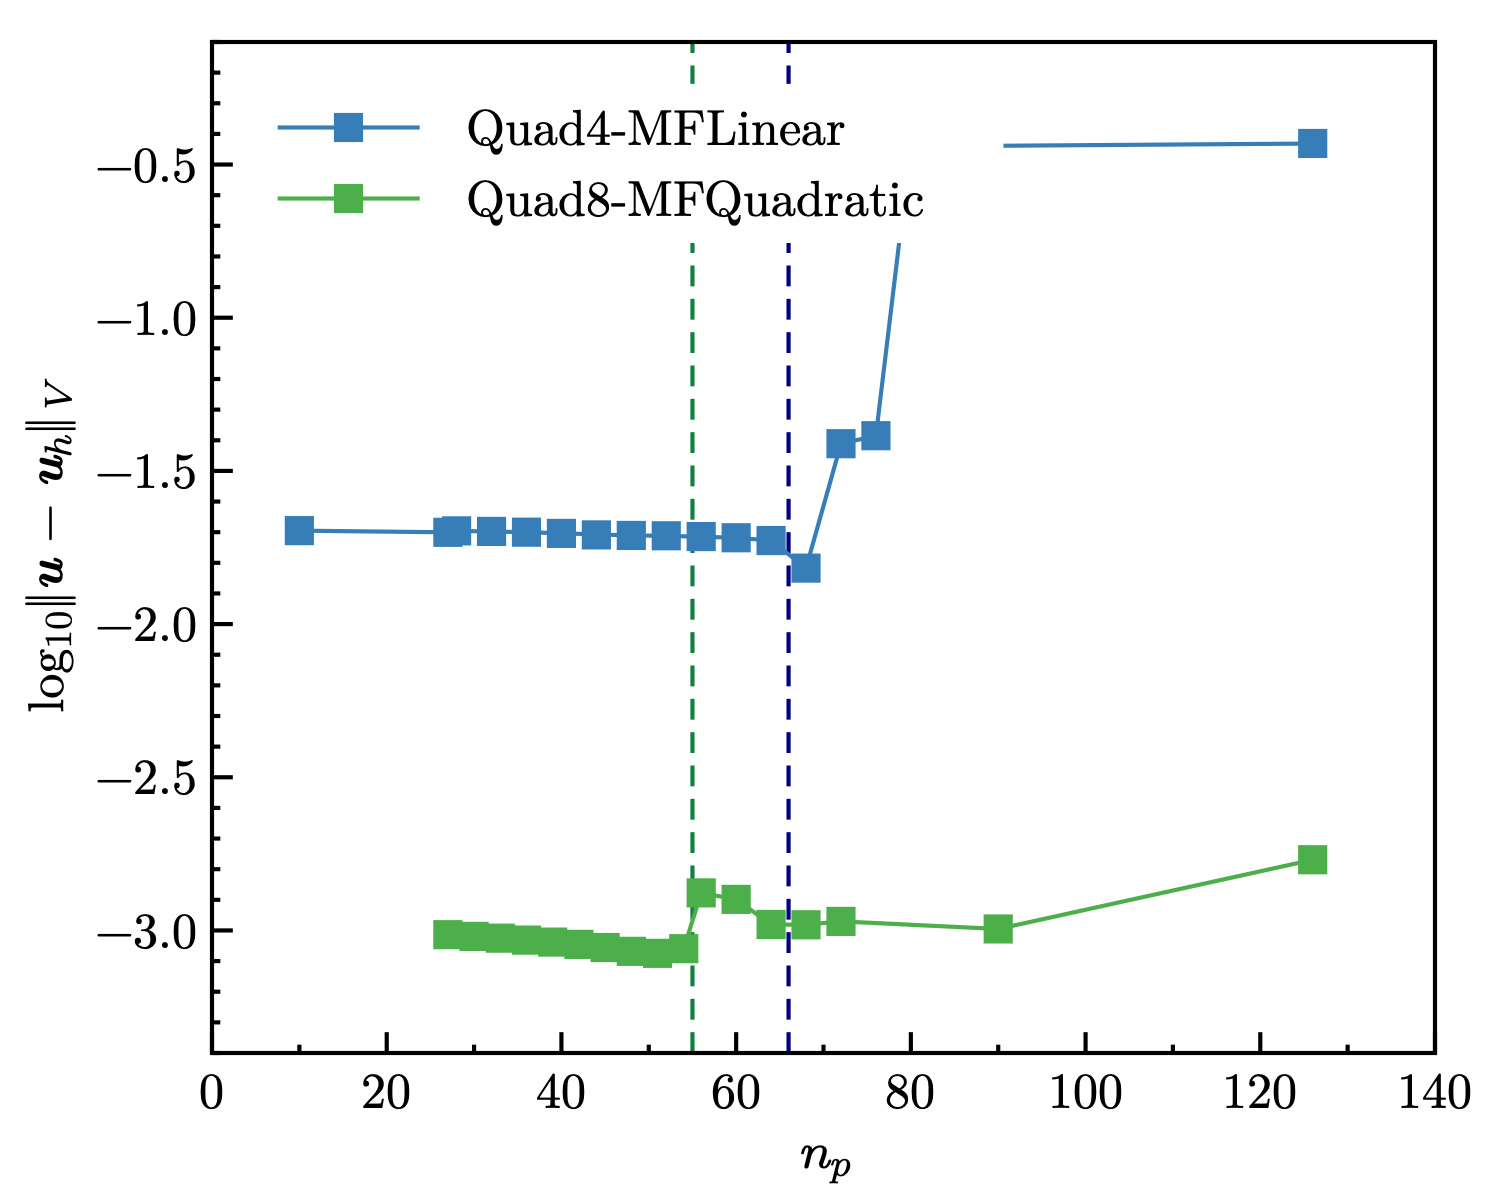
\includegraphics[width=0.45\textwidth]{figures/ch_4/cantilever_4_L2_u.png}
    \phantomcaption\label{cantilever_4_L2_u}
    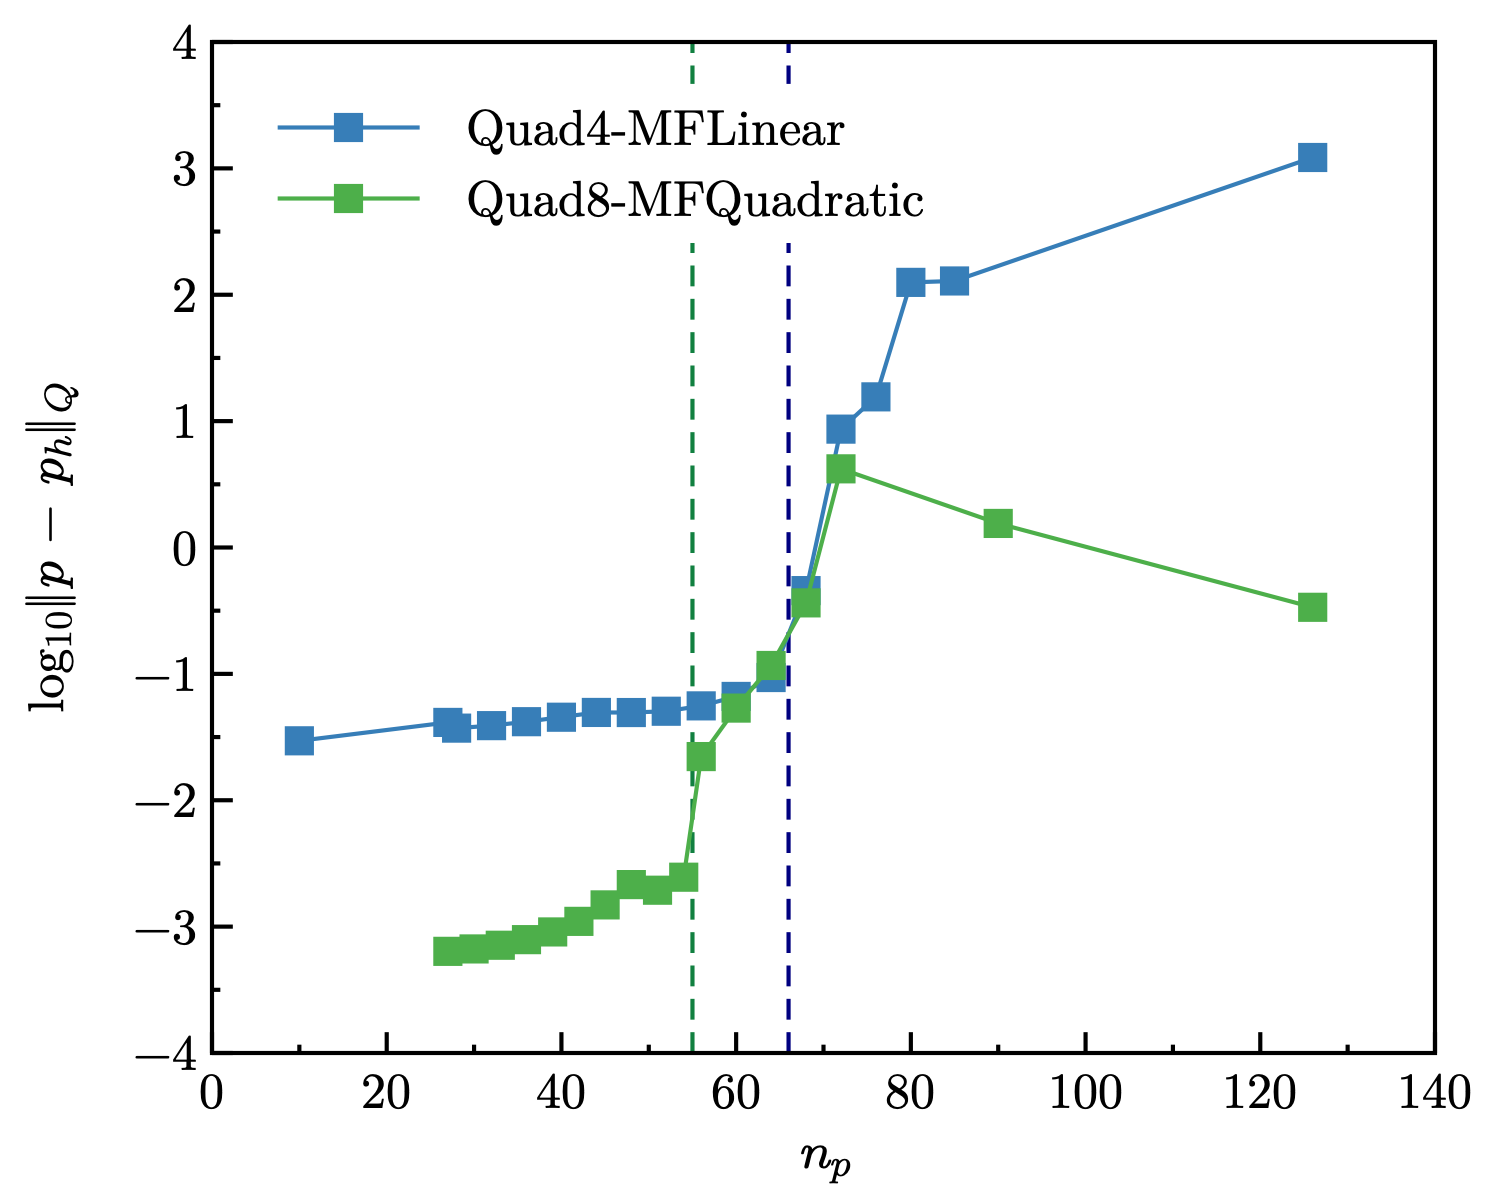
\includegraphics[width=0.45\textwidth]{figures/ch_4/cantilever_4_L2_p.png}
    \phantomcaption\label{cantilever_4_L2_p}
    \end{subcaptiongroup}
    \begin{subcaptiongroup}
    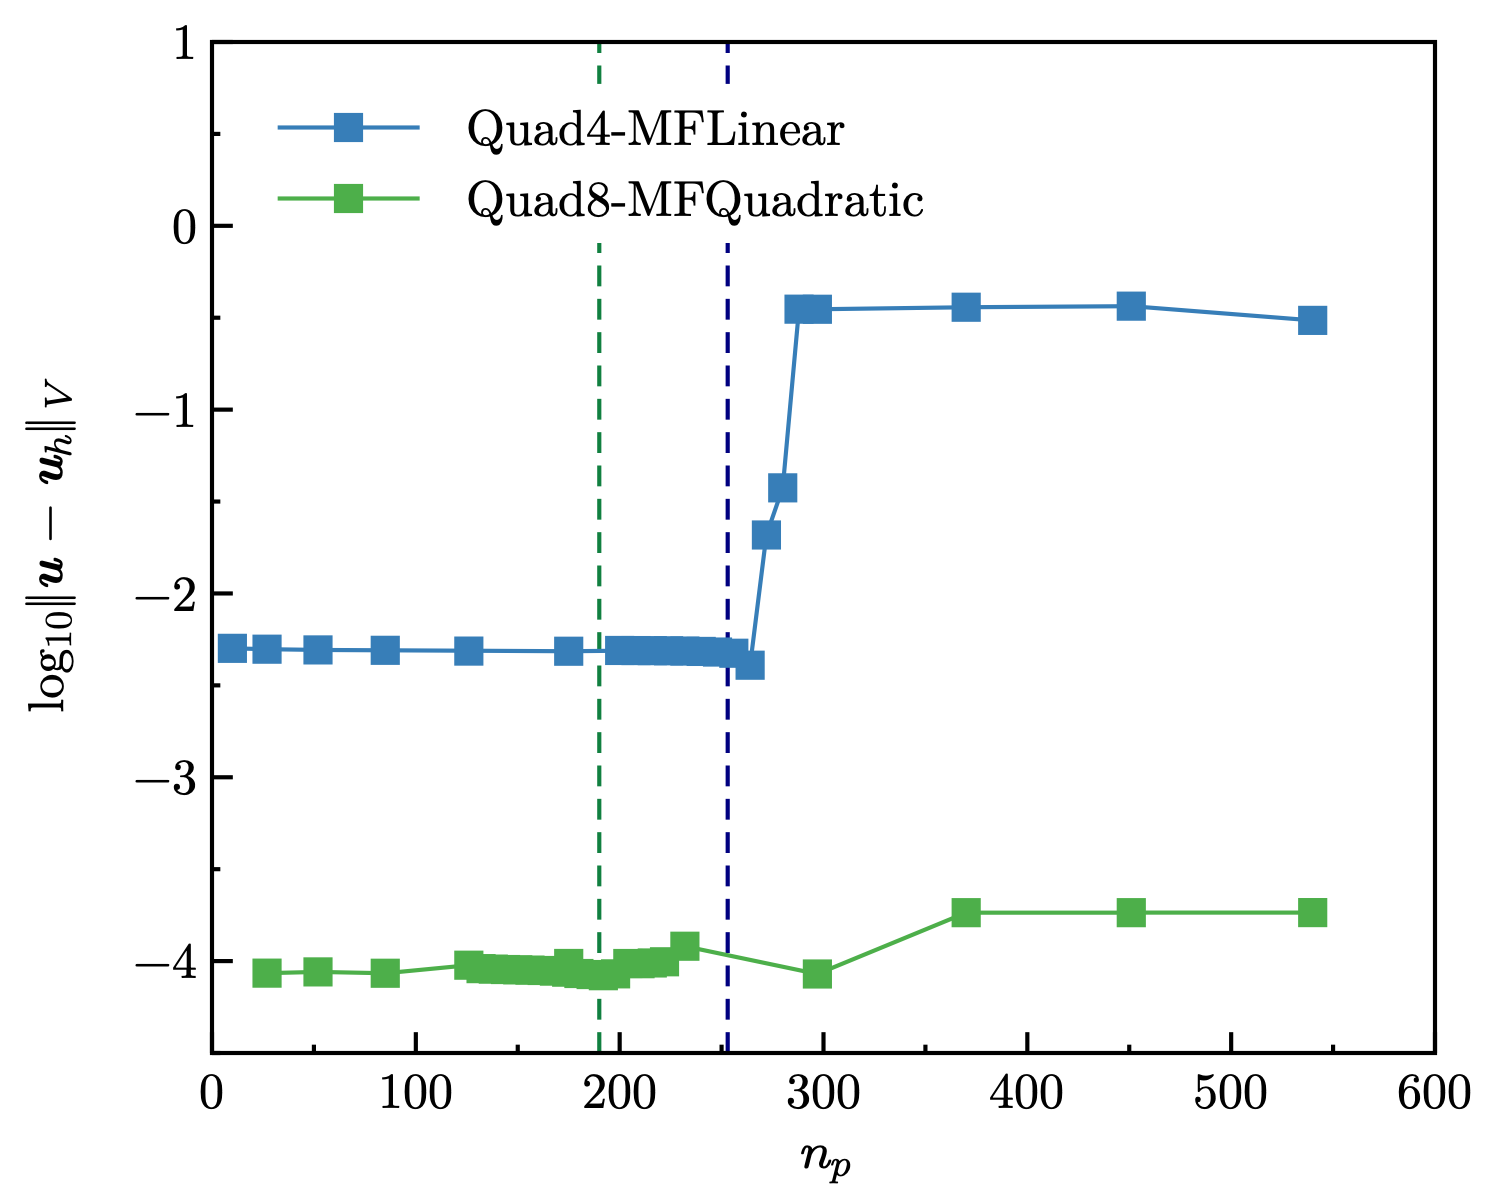
\includegraphics[width=0.45\textwidth]{figures/ch_4/cantilever_8_L2_u.png}
    \phantomcaption\label{cantilever_8_L2_u}
    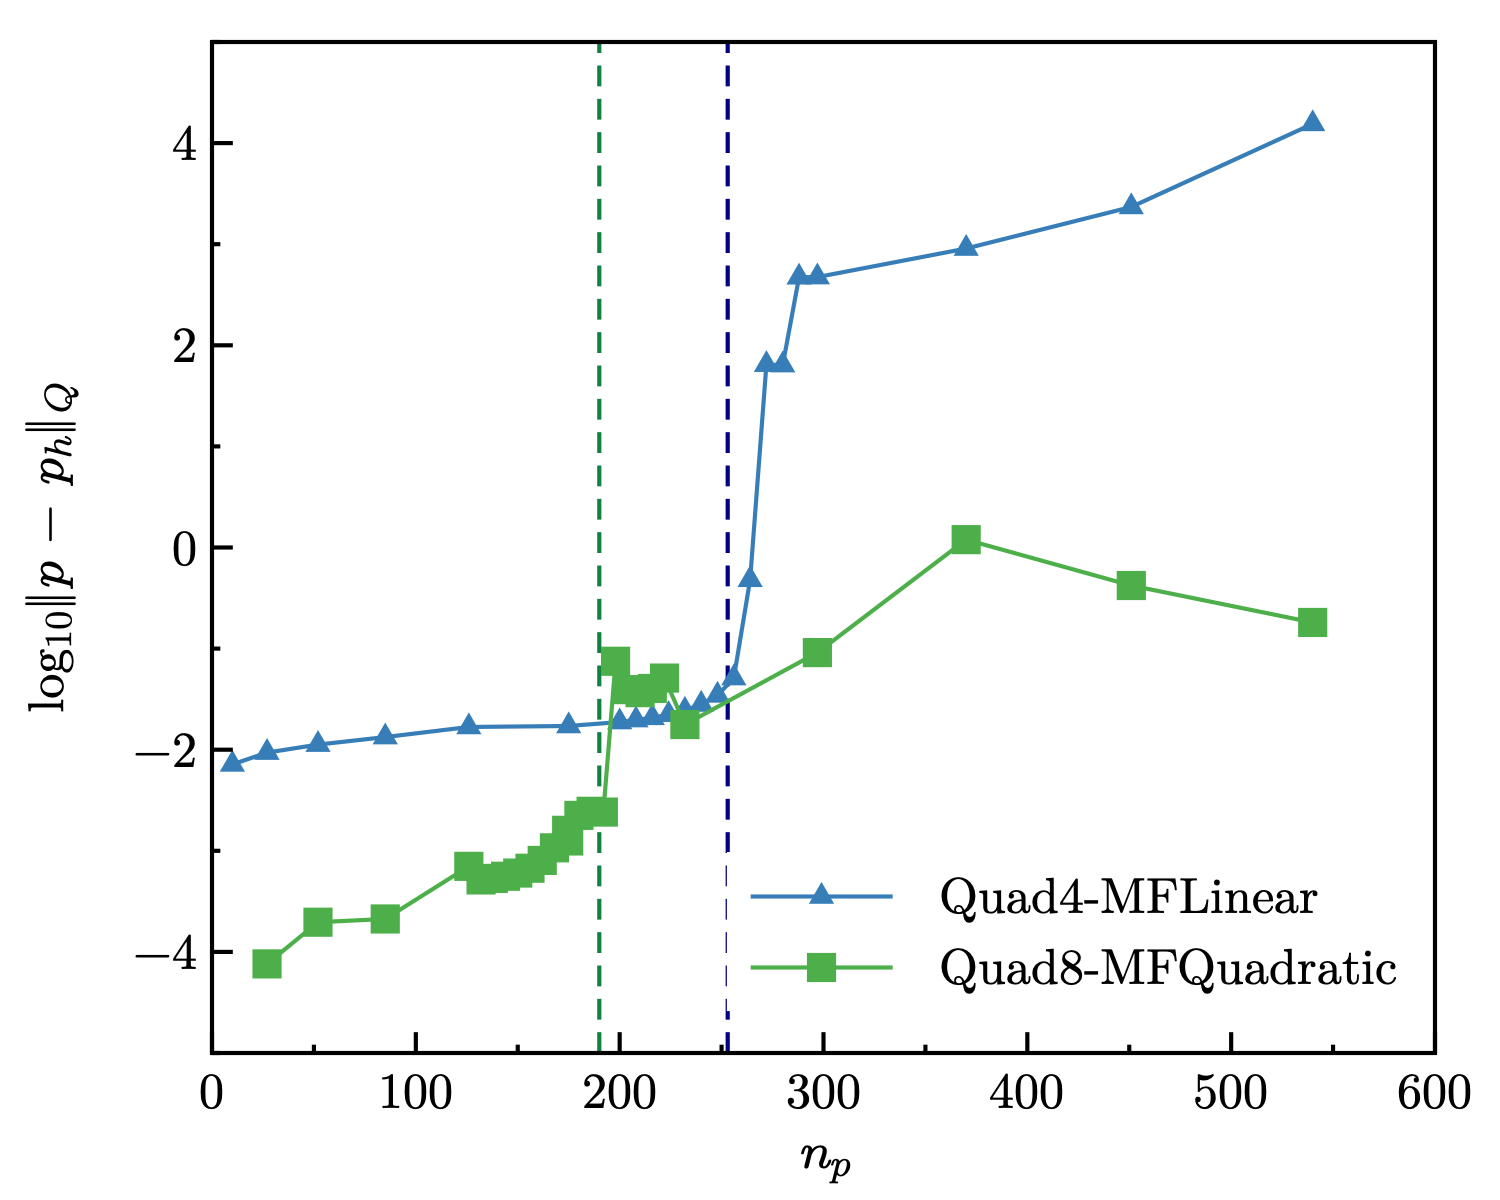
\includegraphics[width=0.45\textwidth]{figures/ch_4/cantilever_8_L2_p.png}
    \phantomcaption\label{cantilever_8_L2_p}
    \end{subcaptiongroup}
    \begin{subcaptiongroup}
    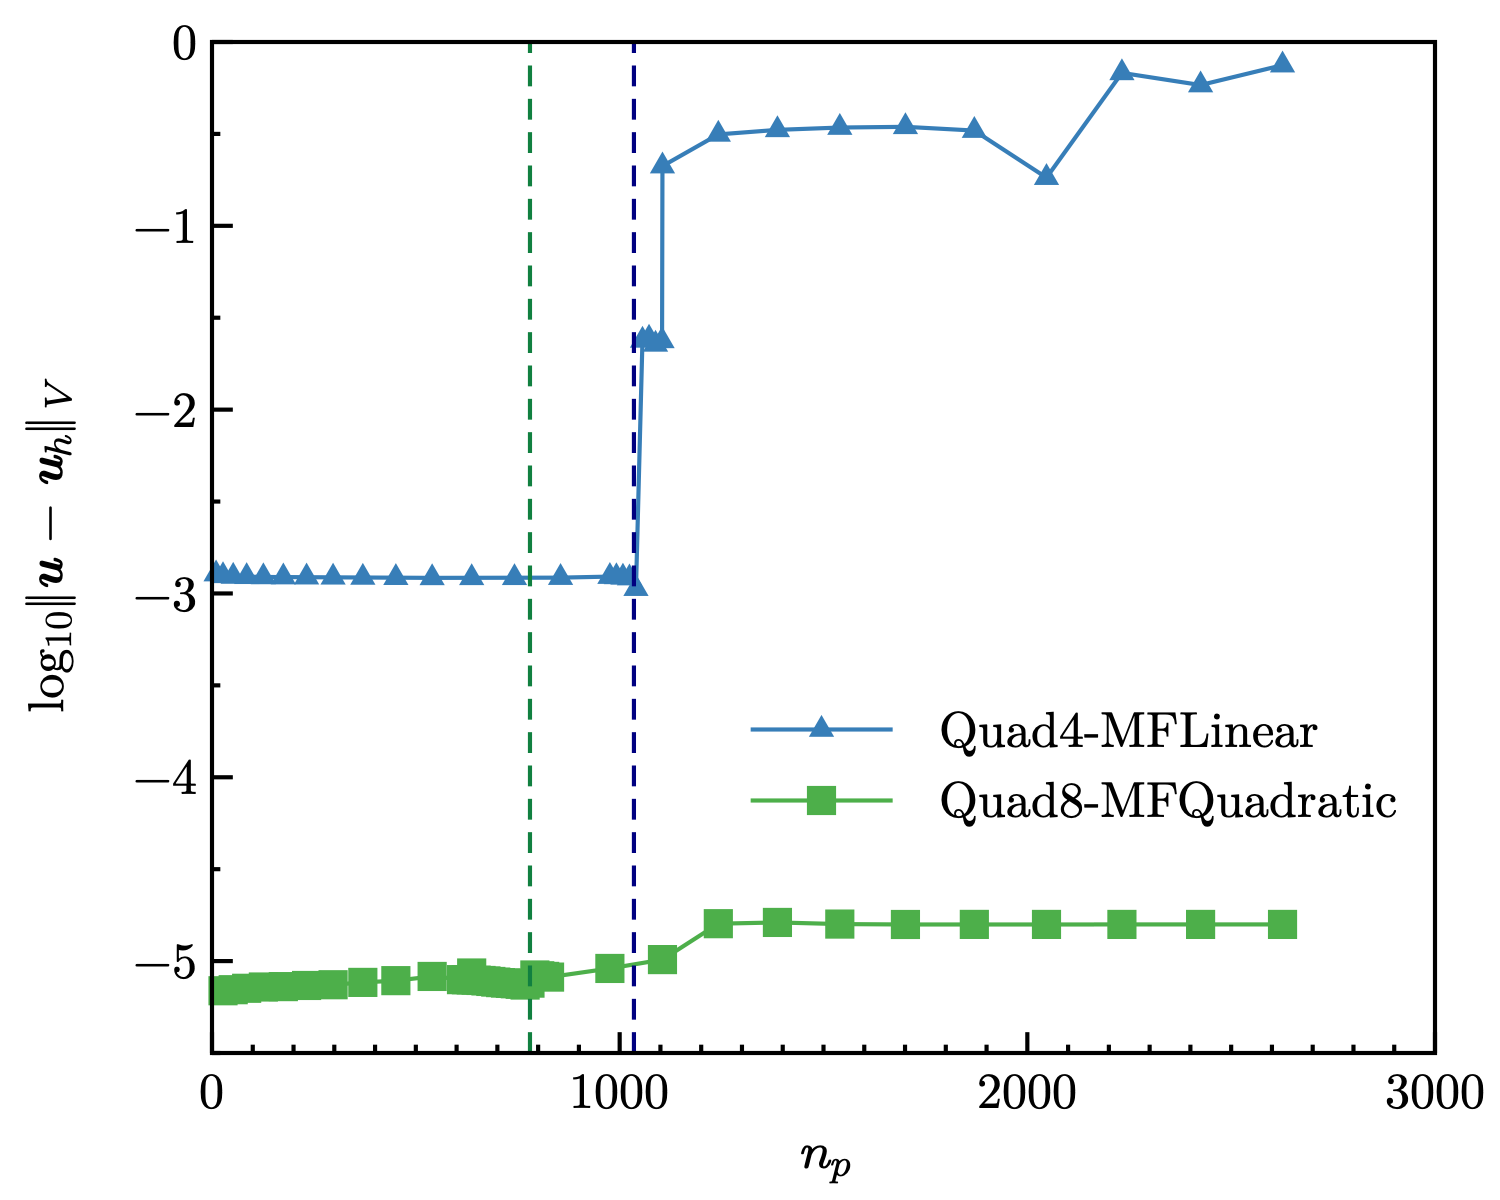
\includegraphics[width=0.45\textwidth]{figures/ch_4/cantilever_16_L2_u.png}
    \phantomcaption\label{cantilever_16_L2_u}
    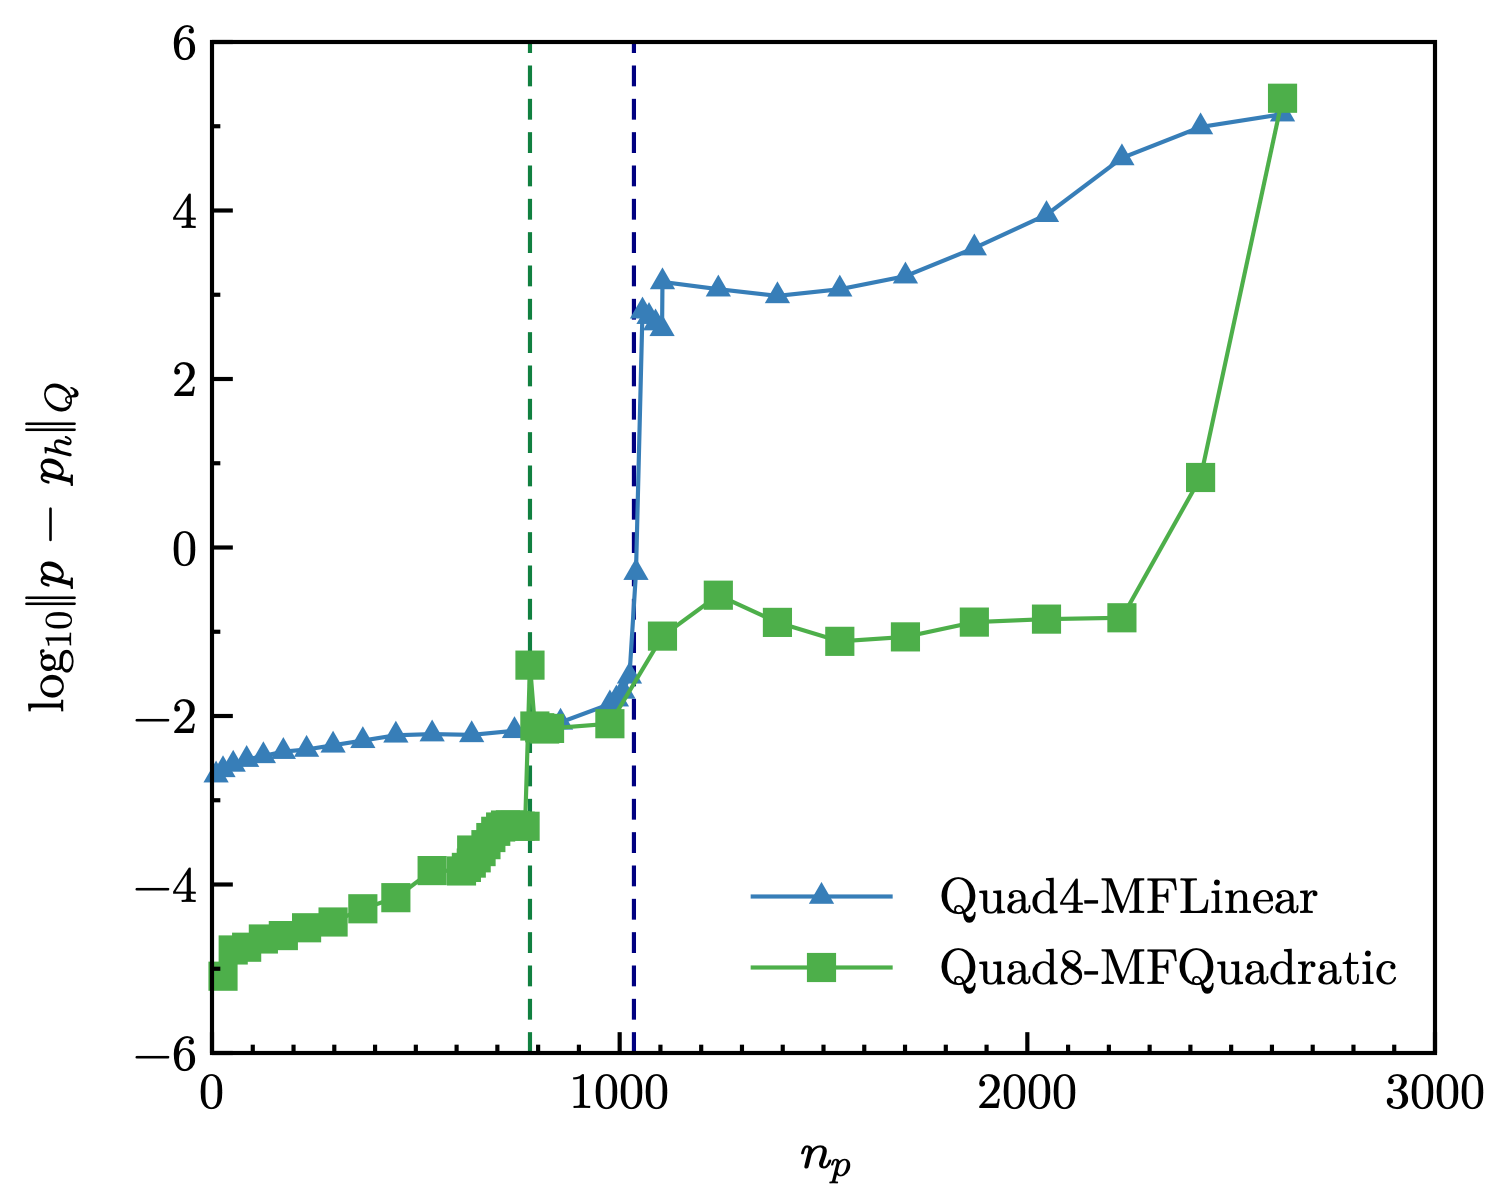
\includegraphics[width=0.45\textwidth]{figures/ch_4/cantilever_16_L2_p.png}
    \phantomcaption\label{cantilever_16_L2_p}
    \end{subcaptiongroup}
    \begin{subcaptiongroup}
    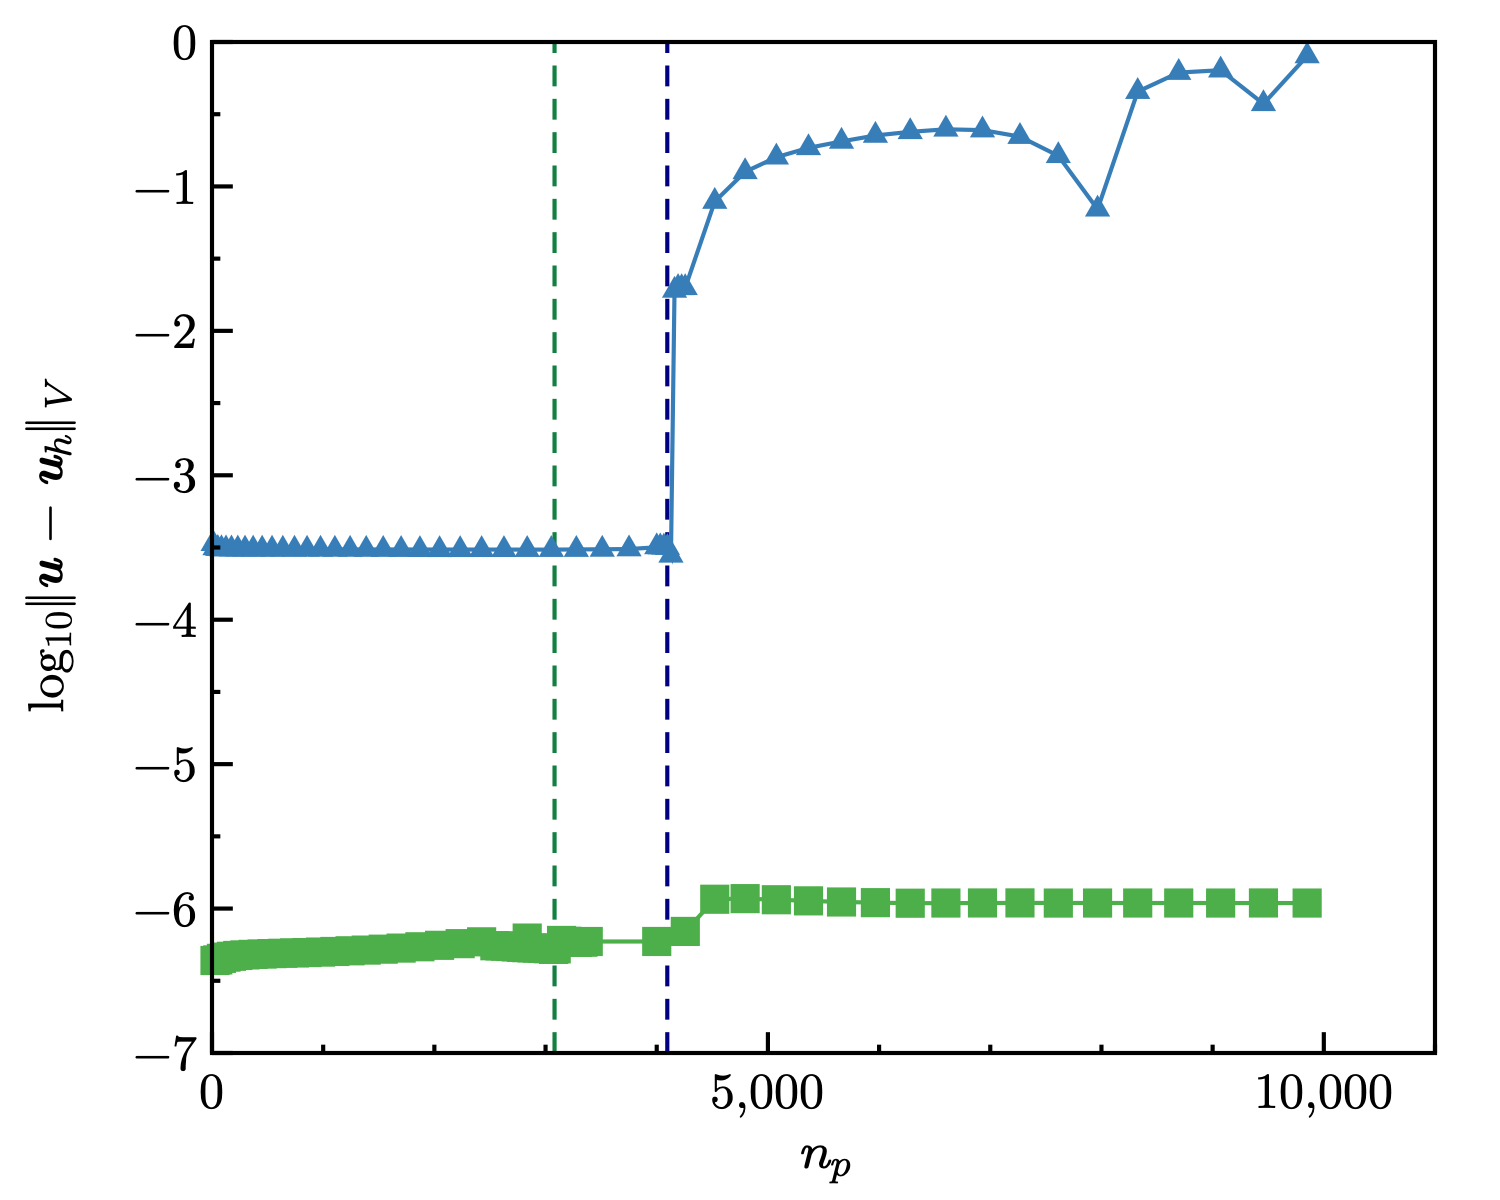
\includegraphics[width=0.45\textwidth]{figures/ch_4/cantilever_32_L2_u.png}
    \phantomcaption\label{cantilever_32_L2_u}
    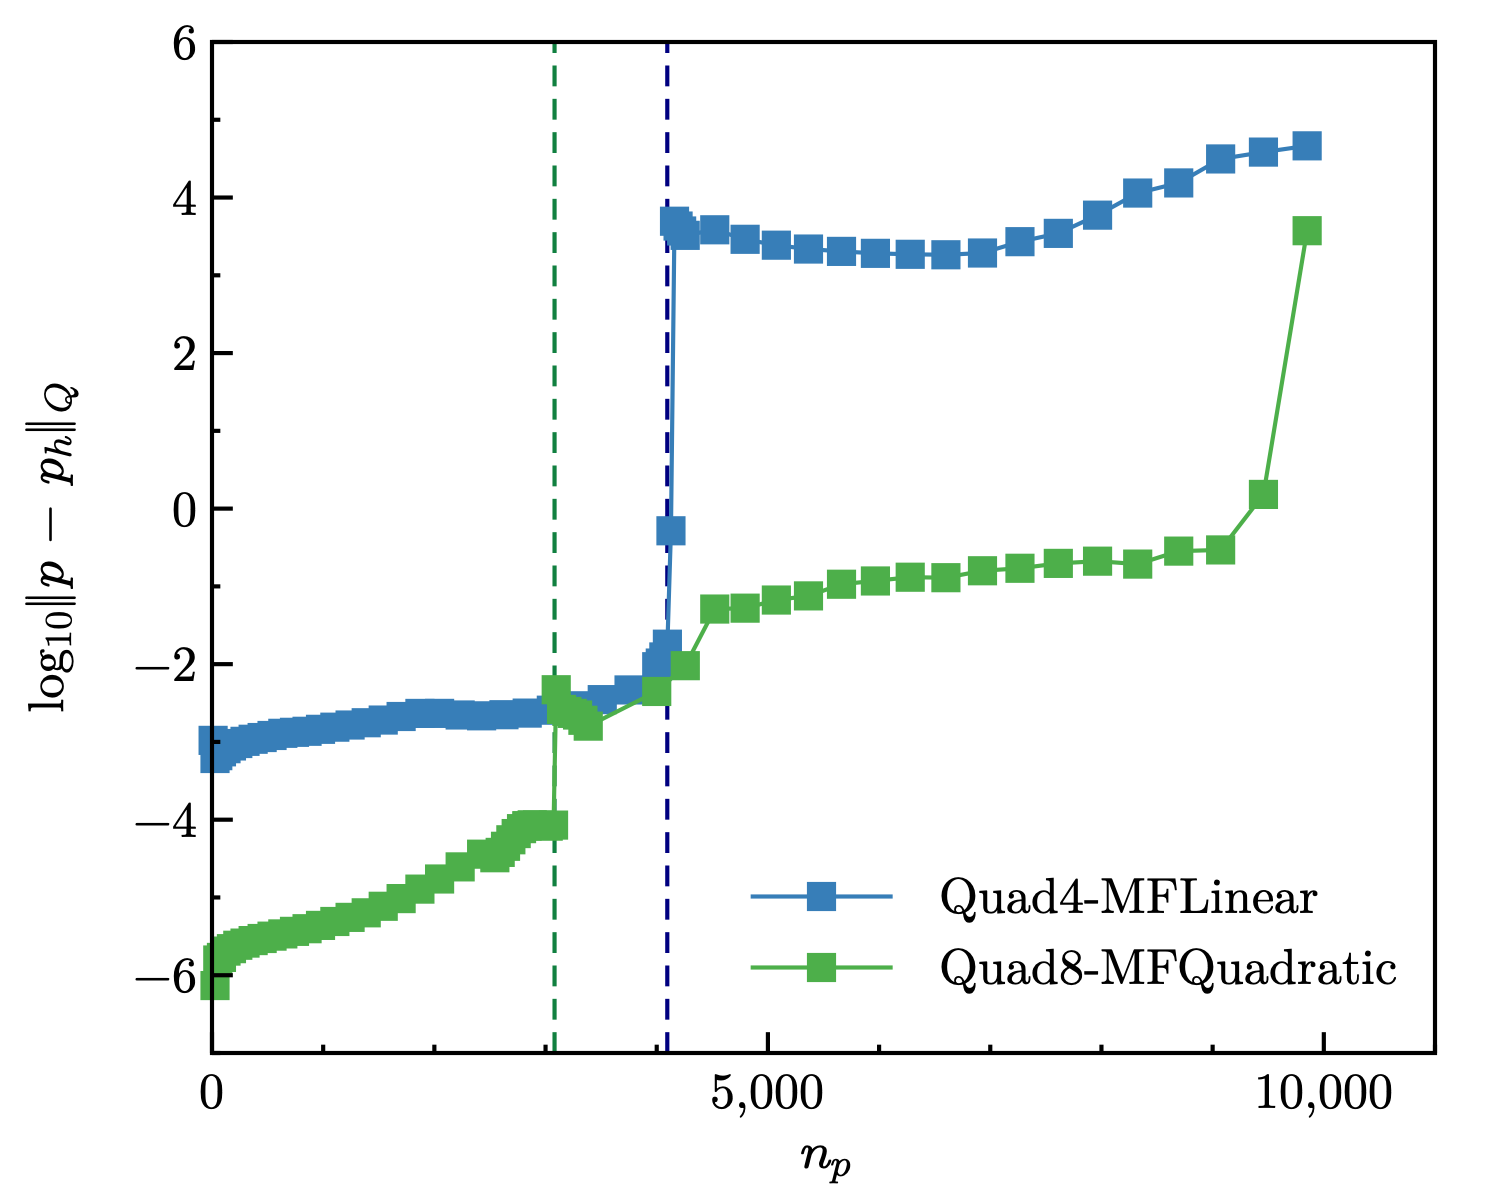
\includegraphics[width=0.45\textwidth]{figures/ch_4/cantilever_32_L2_p.png}
    \phantomcaption\label{cantilever_32_L2_p}
    \end{subcaptiongroup}
\caption{\centering{悬臂梁问题$L2$误差与压力节点数量的关系:\protect\linebreak 
\subref{cantilever_4_L2_u}, \subref{cantilever_4_L2_p} $4\times 4$单元; 
\subref{cantilever_8_L2_u}, \subref{cantilever_8_L2_p} $8\times 8$单元;
\subref{cantilever_16_L2_u},\subref{cantilever_16_L2_p} $16\times 16$单元;
\subref{cantilever_32_L2_u},\subref{cantilever_32_L2_p} $32\times 32$单元;}}
\label{ch_4:fig:cantilever_l2}
\end{figure}

\begin{figure}[!h]
    \centering 
        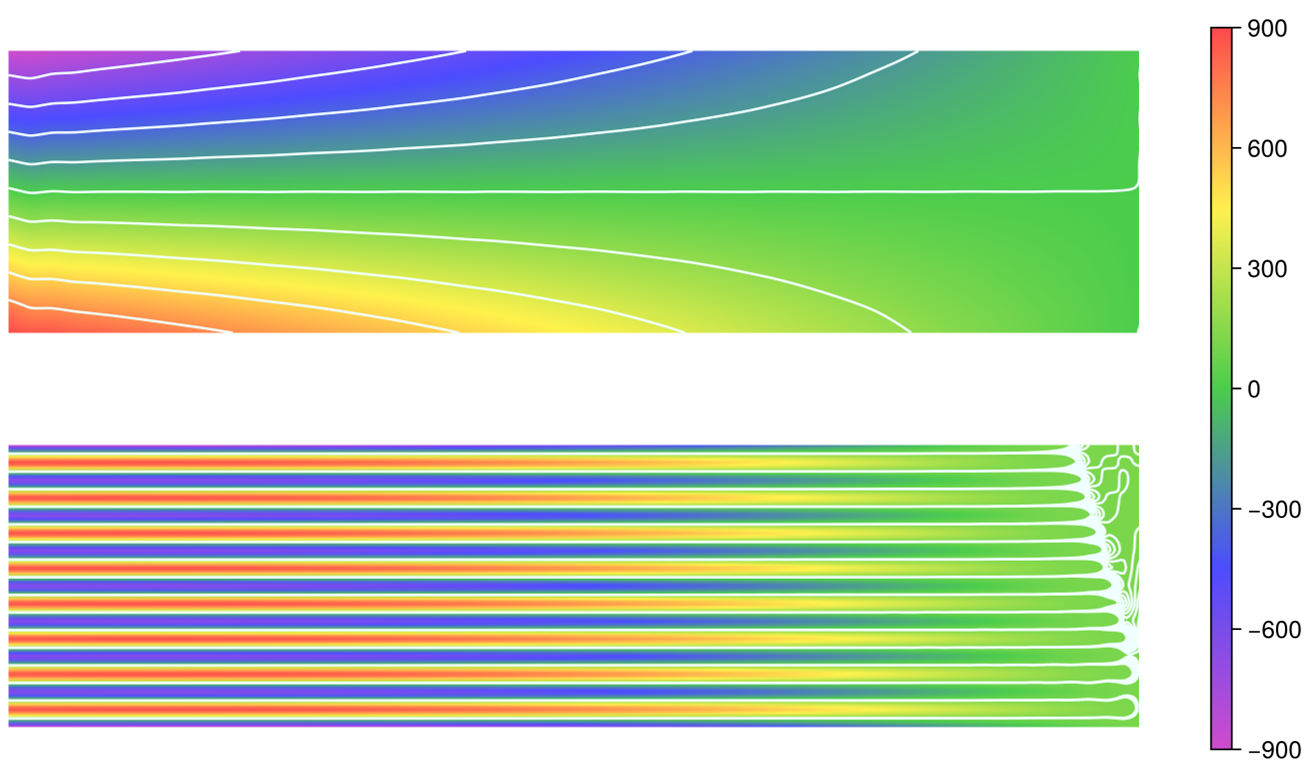
\includegraphics[scale=0.5]{figures/ch_4/cantilever_mix_quad_16.png}
        \caption{悬臂梁问题Quad4单元压力云图(742-1105)}\label{ch_4:fig:cantilever_mix*16}
\end{figure}

\begin{figure}[!h]
    \centering 
        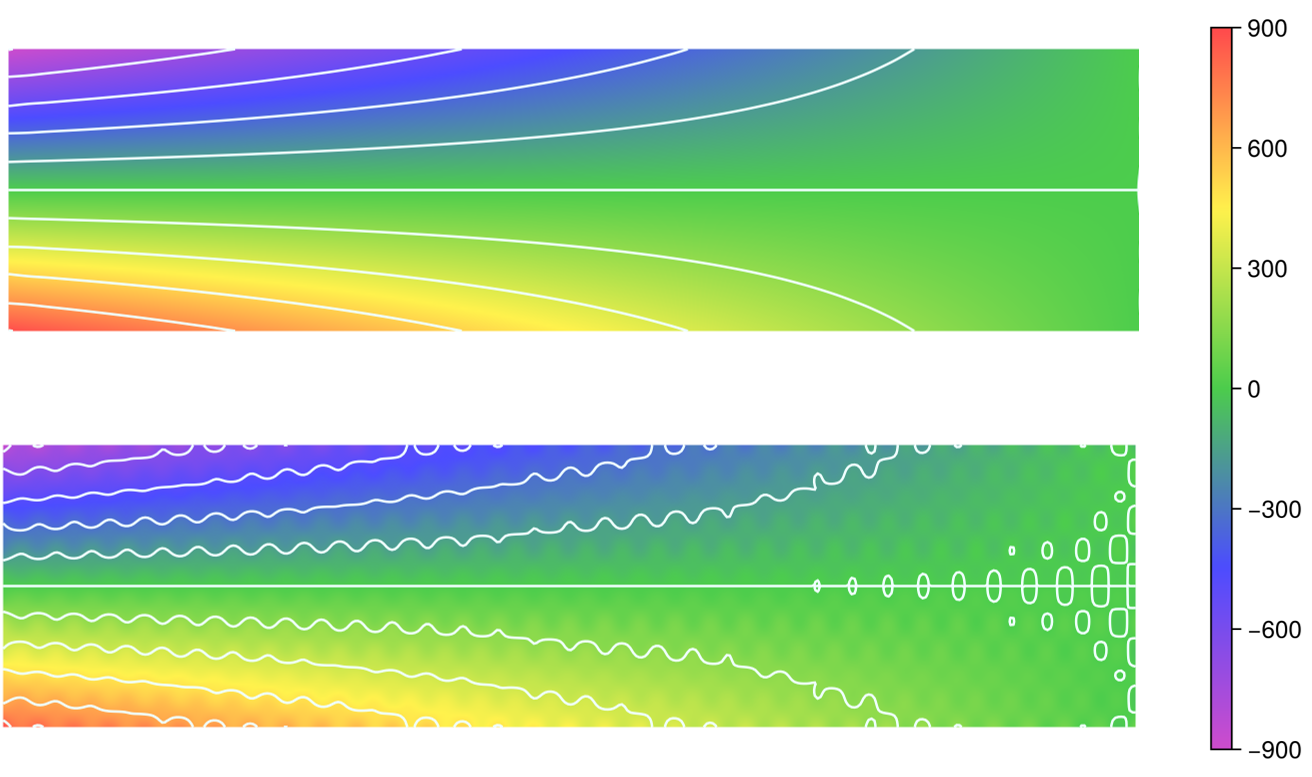
\includegraphics[scale=0.5]{figures/ch_4/cantilever_mix_quad_8.png}
        \caption{悬臂梁问题Quad8单元压力云图(768-780)}\label{ch_4:fig:cantilever_mix_8}
\end{figure}

\subsection{带孔方板问题}

考虑经典的带孔方板问题,如图\ref{ch_4:fig:hole}所示,板的的中心存在一半径为$a=1$的圆形小孔,同时平板的无穷远处沿$x$轴方向施加均布荷载$T=1000$。 板的材料系数为杨氏模量$E=3\times10^6$、泊松比$\nu=0.49999$。根据Michell解可以得到该带孔无限大平板问题的解析解为:
\begin{equation}
    \begin{split}
        u_x(r,\theta)&=\frac{Ta}{8\mu}(\frac{r}{a}(k+1)\cos\theta-\frac{2a^3}{r^3}\cos3\theta    +\frac{2a}{r}((1+k)\cos\theta+\cos3\theta))\\
        u_y(r,\theta)&=\frac{Ta}{8\mu}(\frac{r}{a}(k-3)\sin\theta-\frac{2a^3}{r^3}\sin3\theta    +\frac{2a}{r}((1-k)\sin\theta+\sin3\theta))  
    \end{split}
\end{equation}
其中,$k$和$\mu$分别为:
\begin{equation}
    \begin{split}
        k=\frac{3-\nu}{1+\nu}\quad \text{,}\mu=\frac{E}{2(1+\nu)}
    \end{split}
\end{equation}
与之相对应的应力分量为:
\begin{equation}
\begin{split}
    \sigma_{xx}&=T(1-\frac{a^2}{r^2}(\frac{3}{2}\cos2\theta+\cos4\theta)+\frac{3a^4}{2r^4}\cos4\theta)\\
    \sigma_{yy}&=-T(\frac{a^2}{r^2}(\frac{1}{2}\cos2\theta-\cos4\theta)+\frac{3a^4}{2r^4}\cos4\theta)\\
    \sigma_{xy}&=-T(\frac{a^2}{r^2}(\frac{1}{2}\sin2\theta+\sin4\theta)-\frac{3a^4}{2r^4}\sin4\theta)\\
\end{split}
\end{equation}

\begin{figure}[!h]
    \centering 
        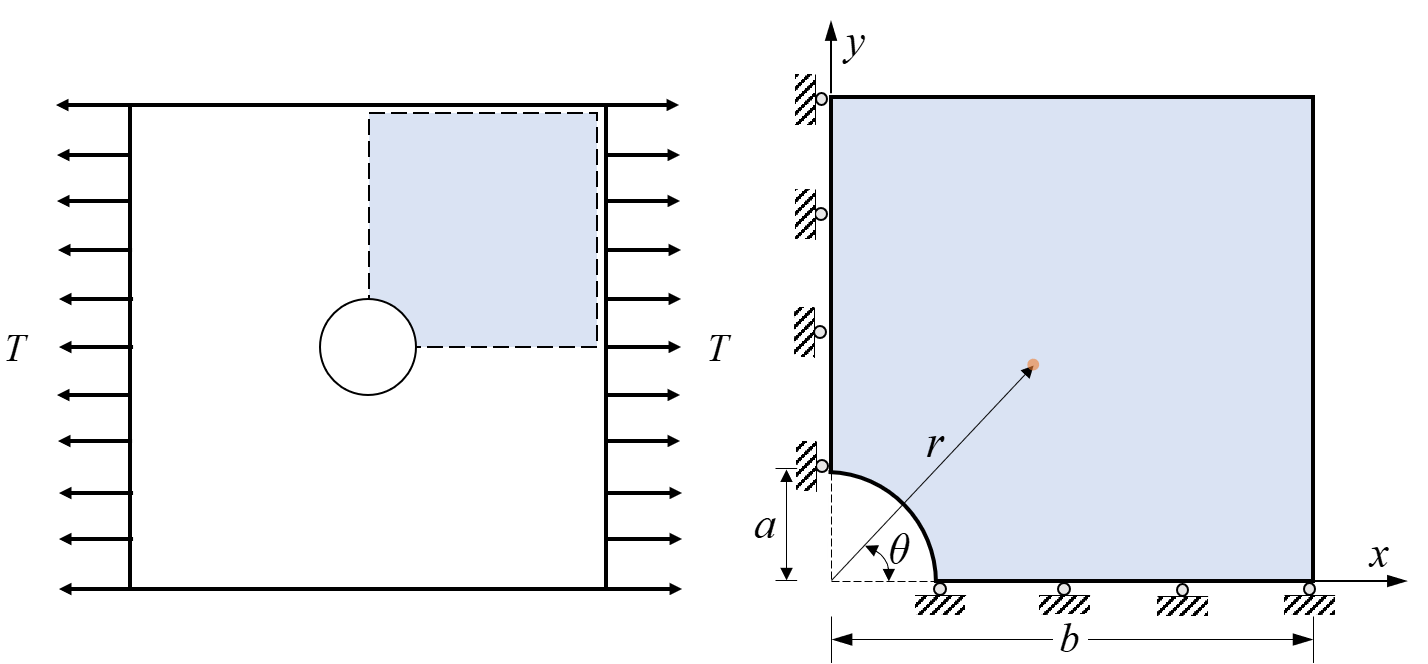
\includegraphics[scale=0.5]{figures/ch_4/hole.png}
        \caption{带孔方板问题模型}\label{ch_4:fig:hole}
\end{figure}
\begin{figure}[H]
    \centering
    \begin{subcaptiongroup}
    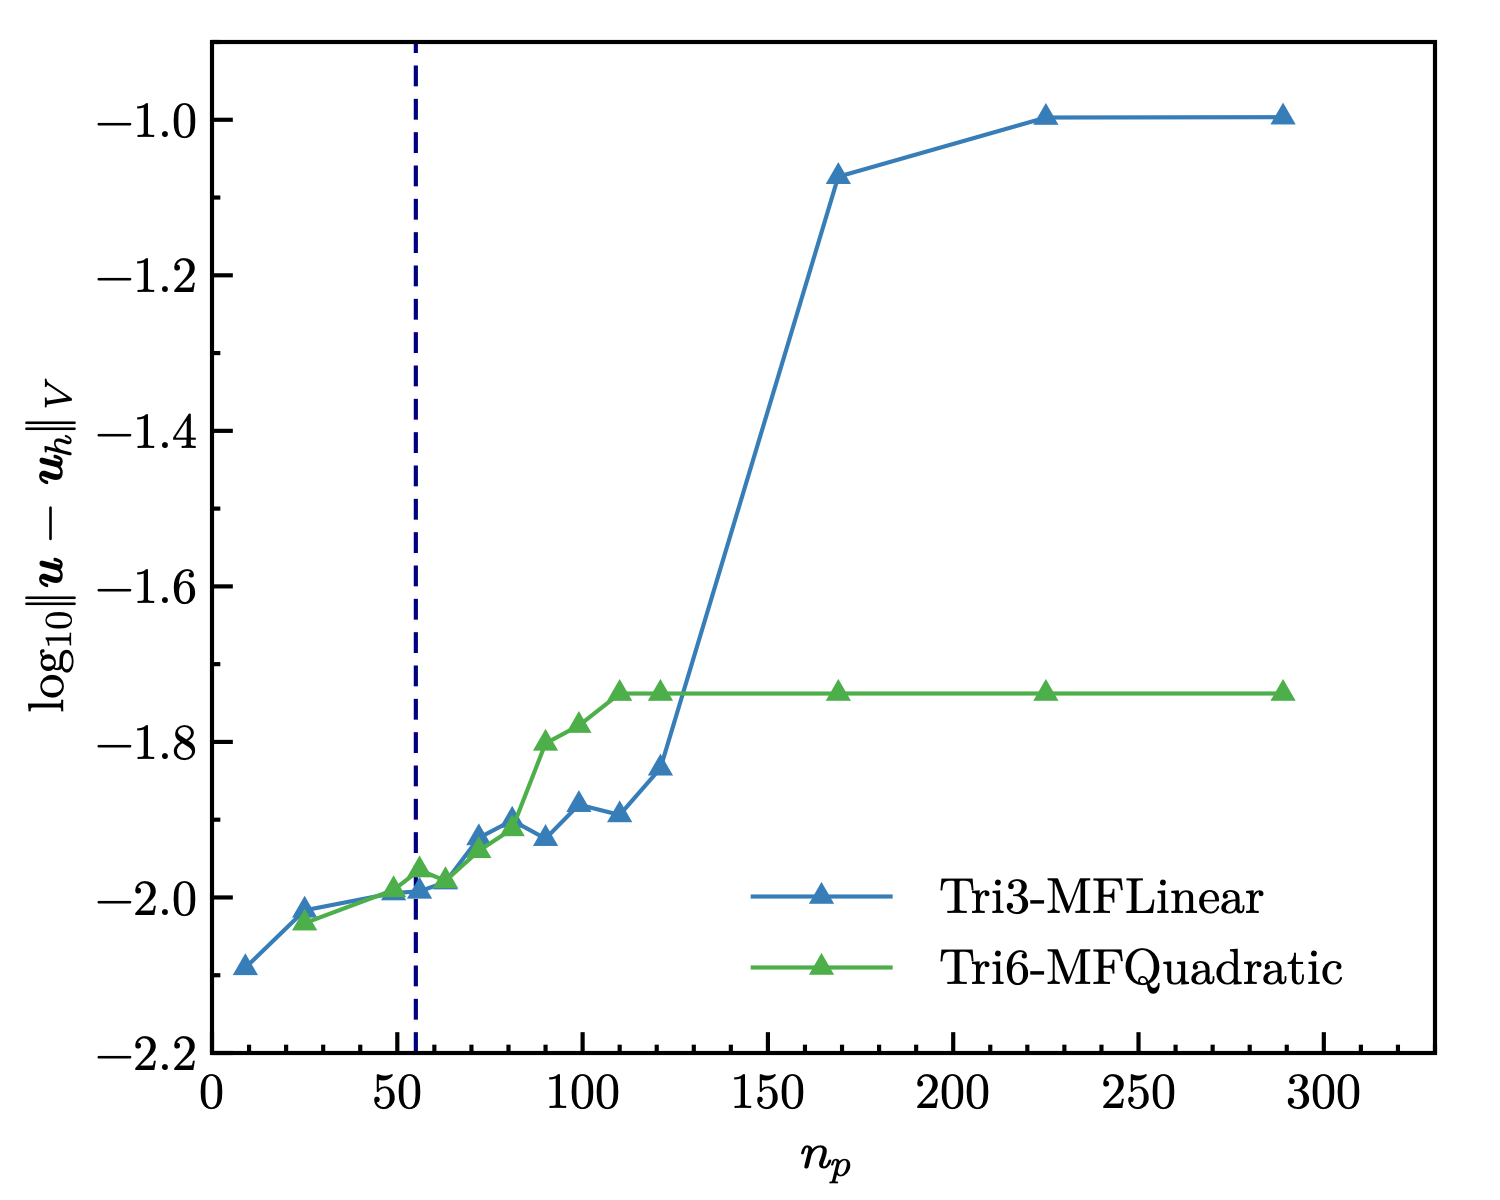
\includegraphics[width=0.45\textwidth]{figures/ch_4/plate_with_hole_4_L2_u.png}
    \phantomcaption\label{hole_4_L2_u}
    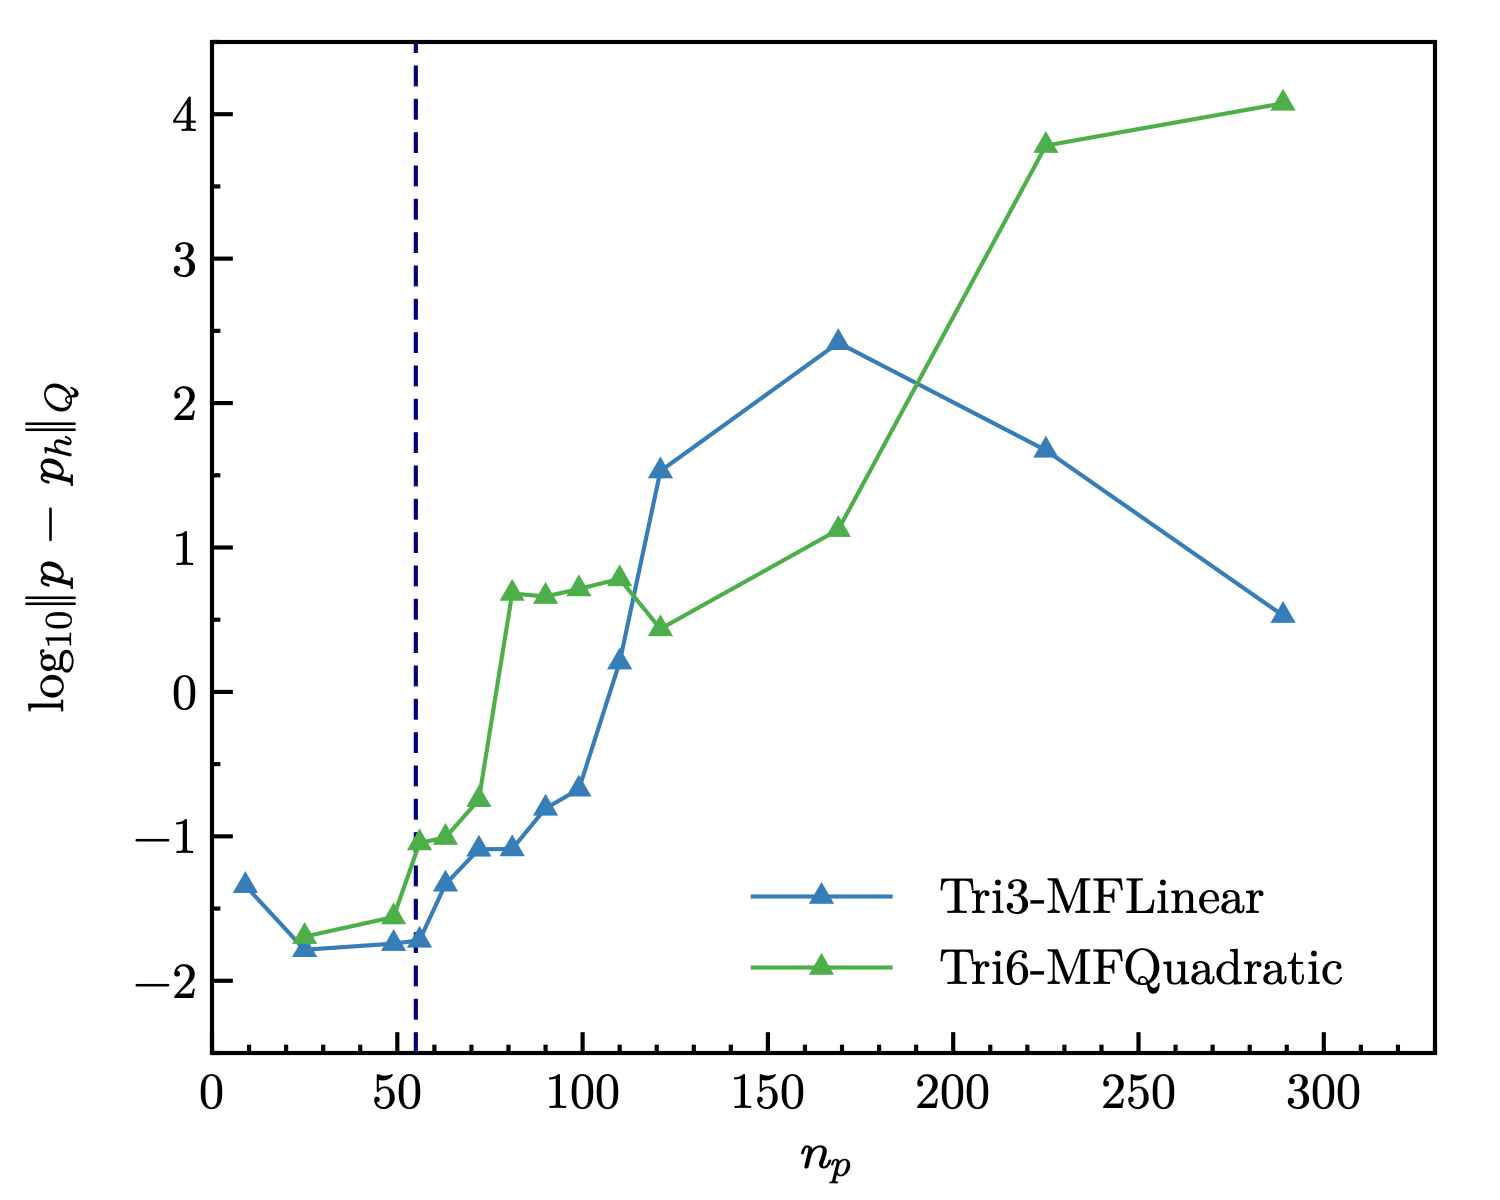
\includegraphics[width=0.45\textwidth]{figures/ch_4/plate_with_hole_4_L2_p.png}
    \phantomcaption\label{hole_4_L2_p}
    \end{subcaptiongroup}
    \begin{subcaptiongroup}
    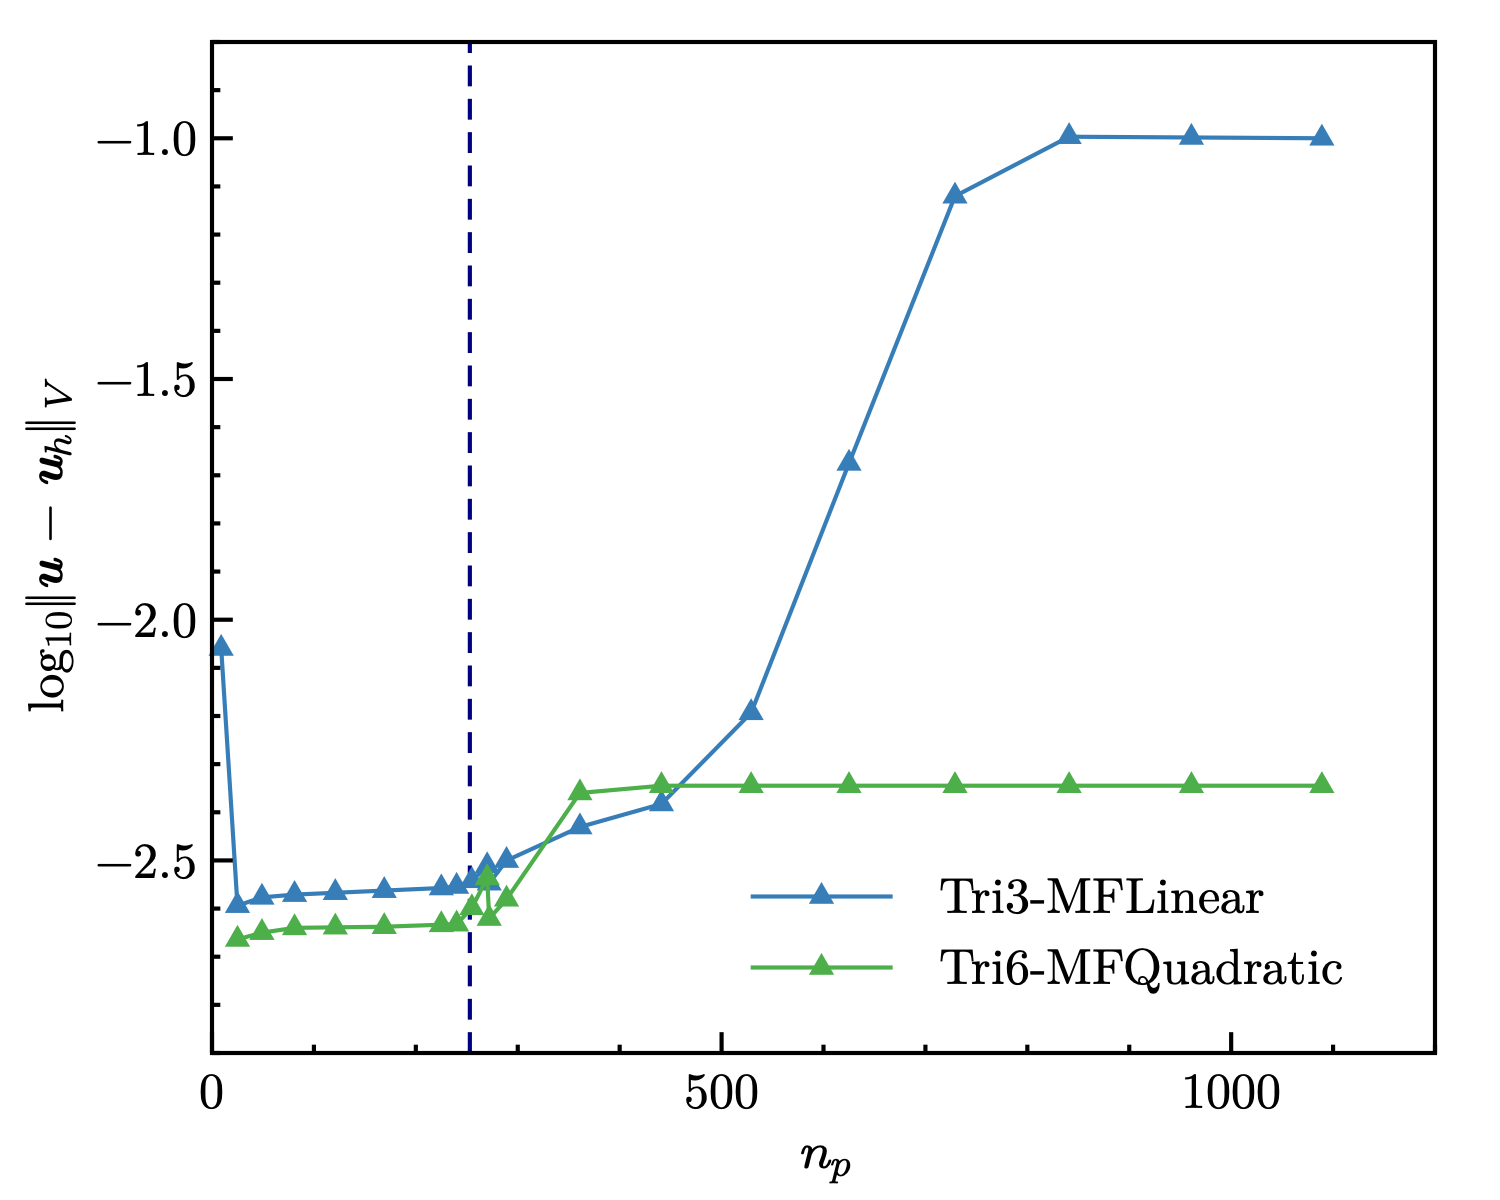
\includegraphics[width=0.45\textwidth]{figures/ch_4/plate_with_hole_8_L2_u.png}
    \phantomcaption\label{hole_8_L2_u}
    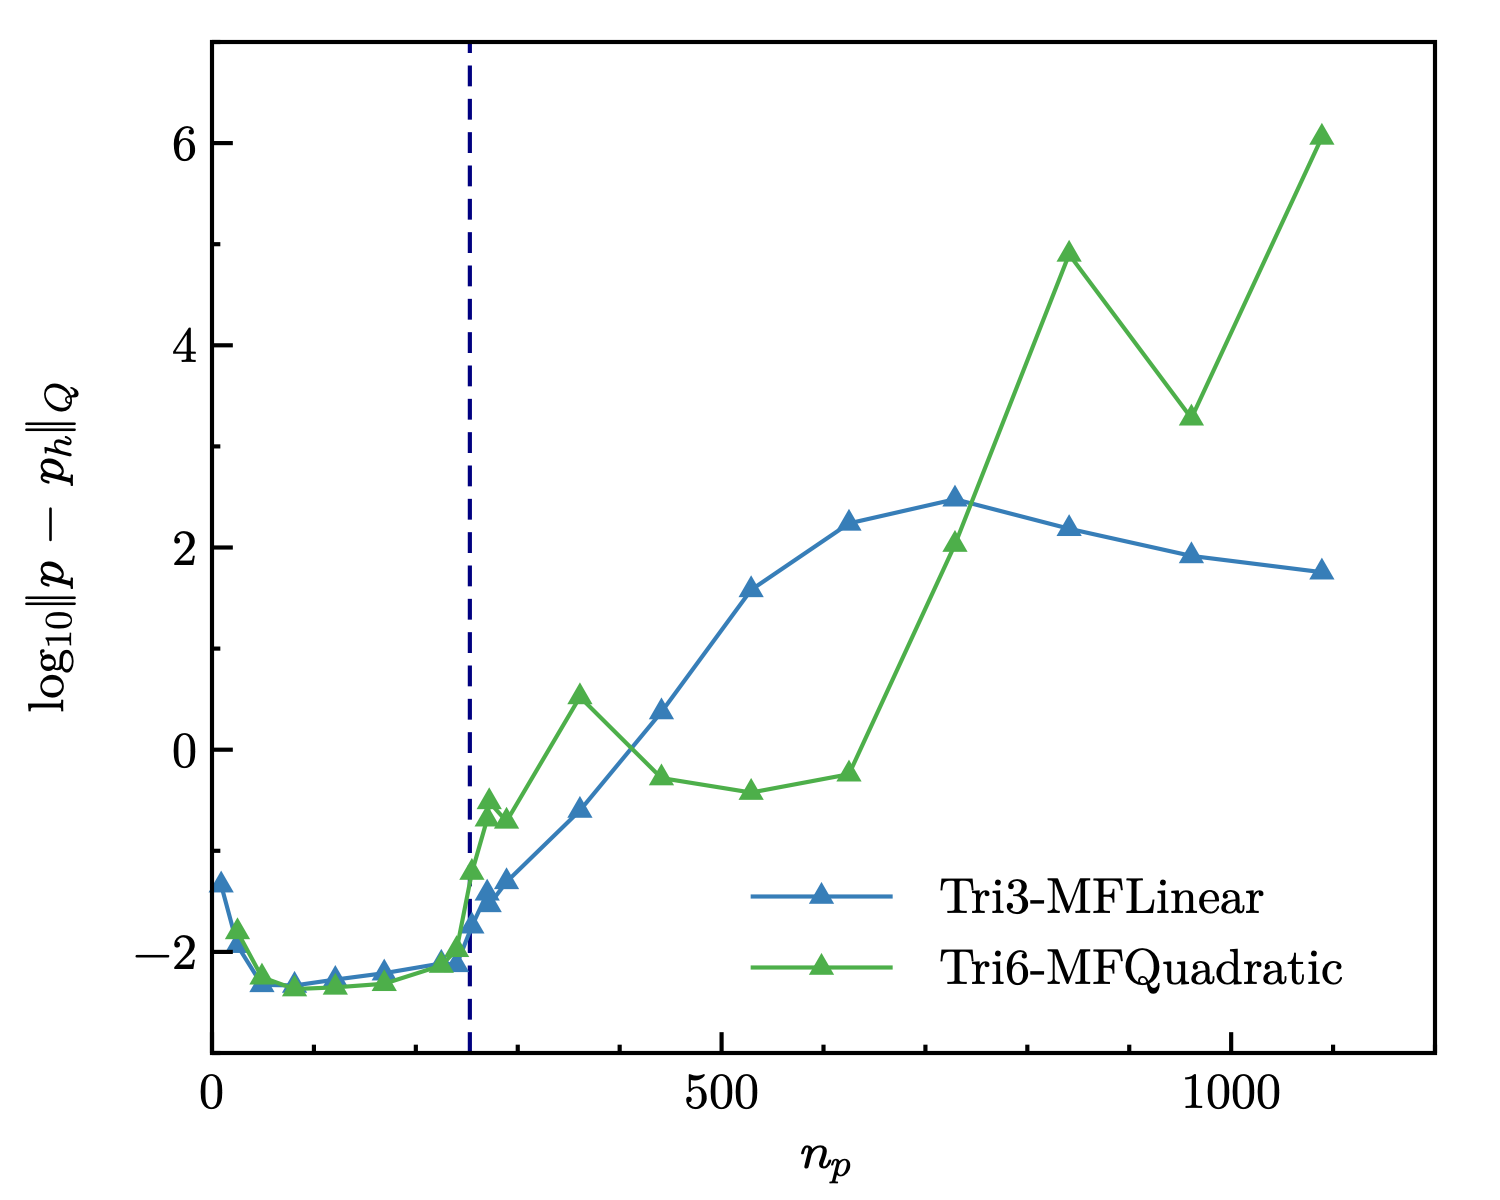
\includegraphics[width=0.45\textwidth]{figures/ch_4/plate_with_hole_8_L2_p.png}
    \phantomcaption\label{hole_8_L2_p}
    \end{subcaptiongroup}
    \begin{subcaptiongroup}
    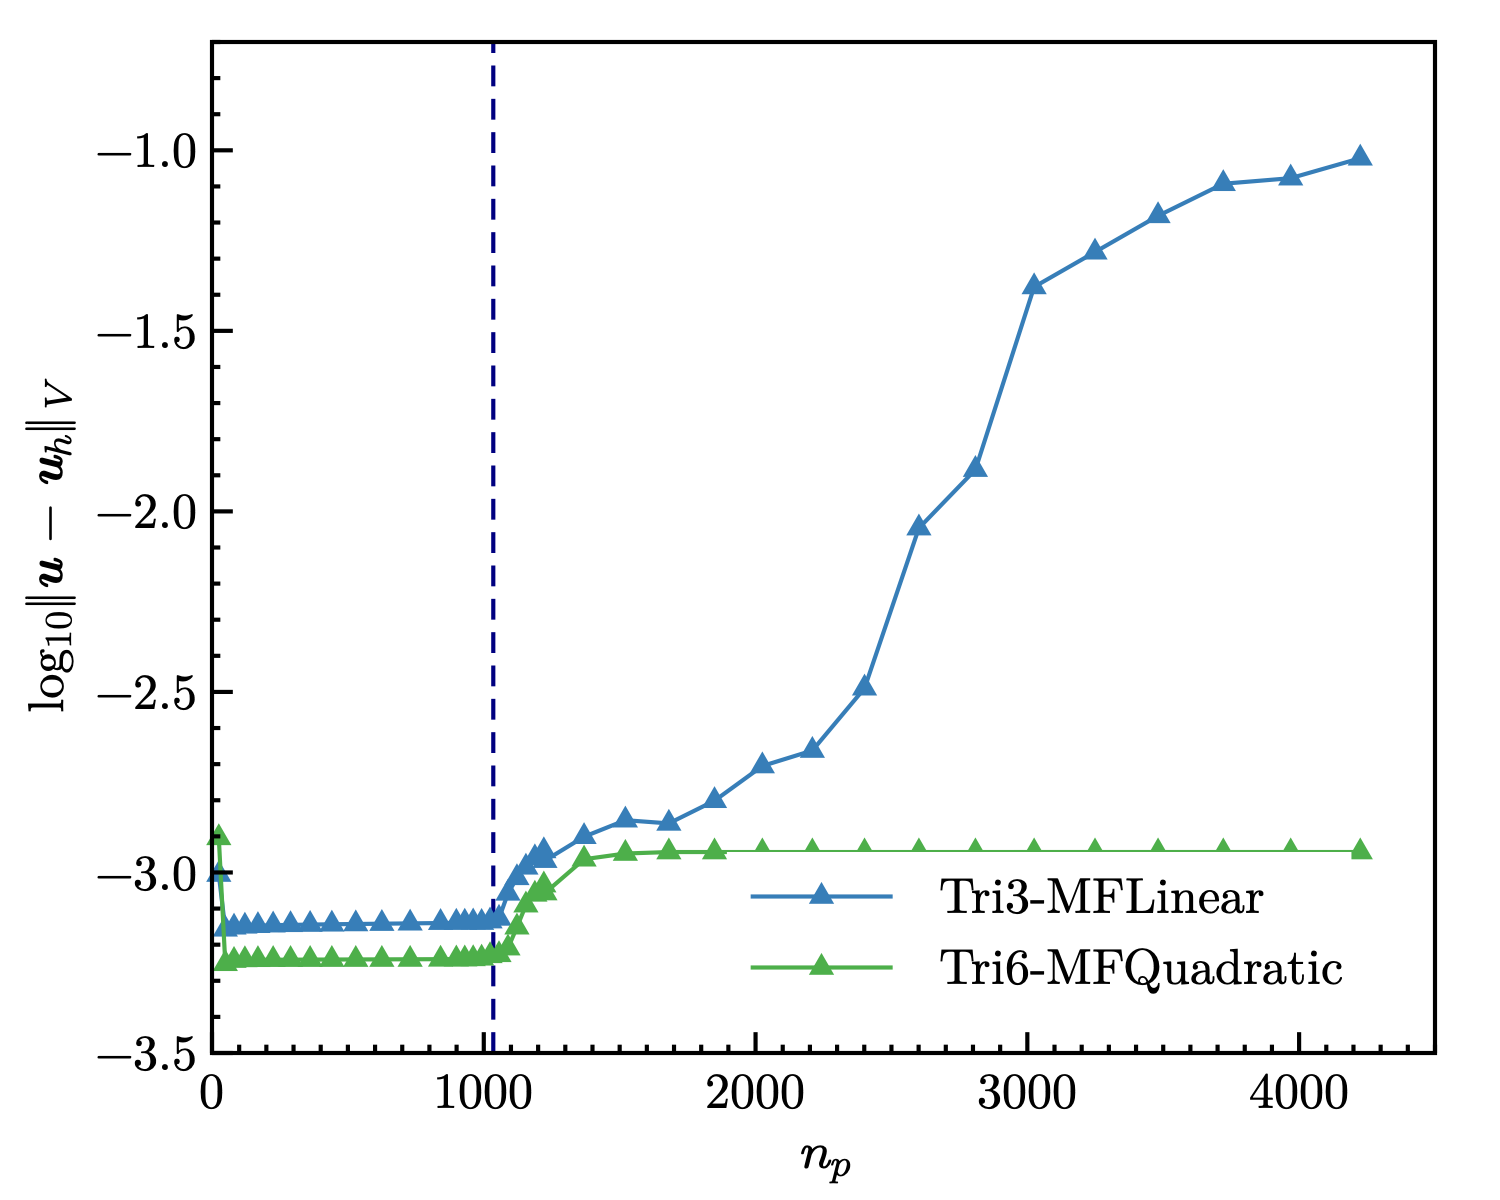
\includegraphics[width=0.45\textwidth]{figures/ch_4/plate_with_hole_16_L2_u.png}
    \phantomcaption\label{hole_16_L2_u}
    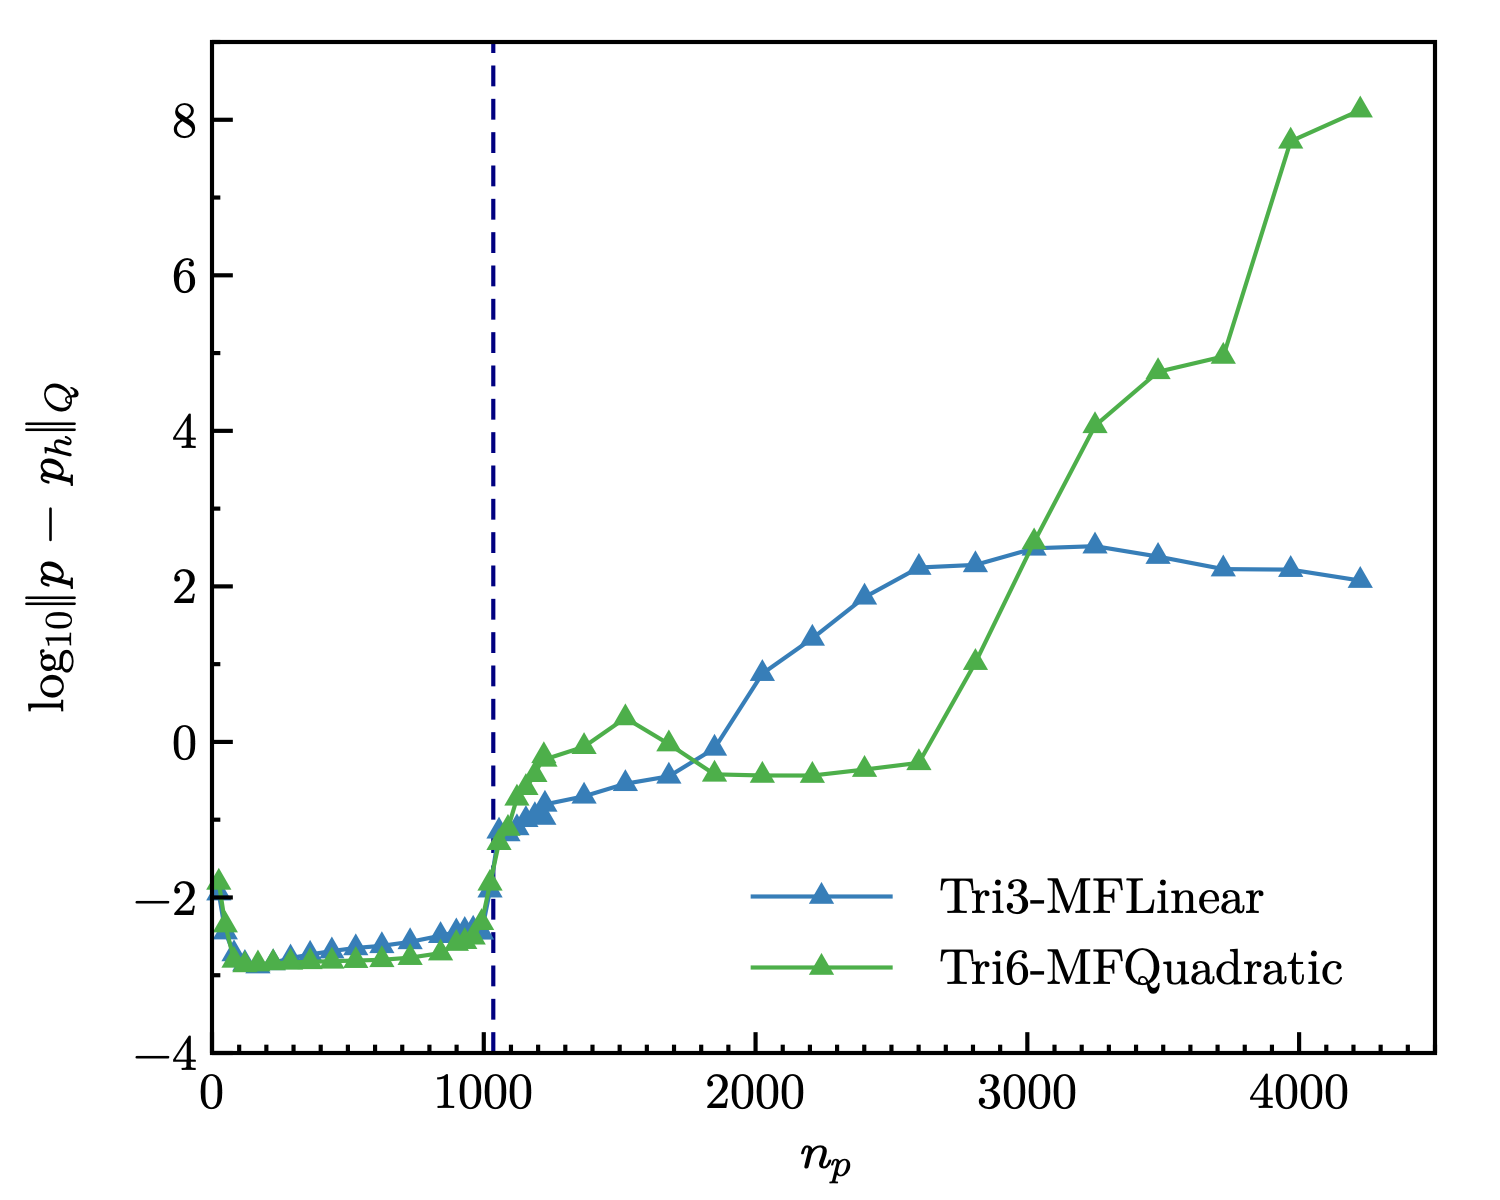
\includegraphics[width=0.45\textwidth]{figures/ch_4/plate_with_hole_16_L2_p.png}
    \phantomcaption\label{hole_16_L2_p}
    \end{subcaptiongroup}
    \begin{subcaptiongroup}
    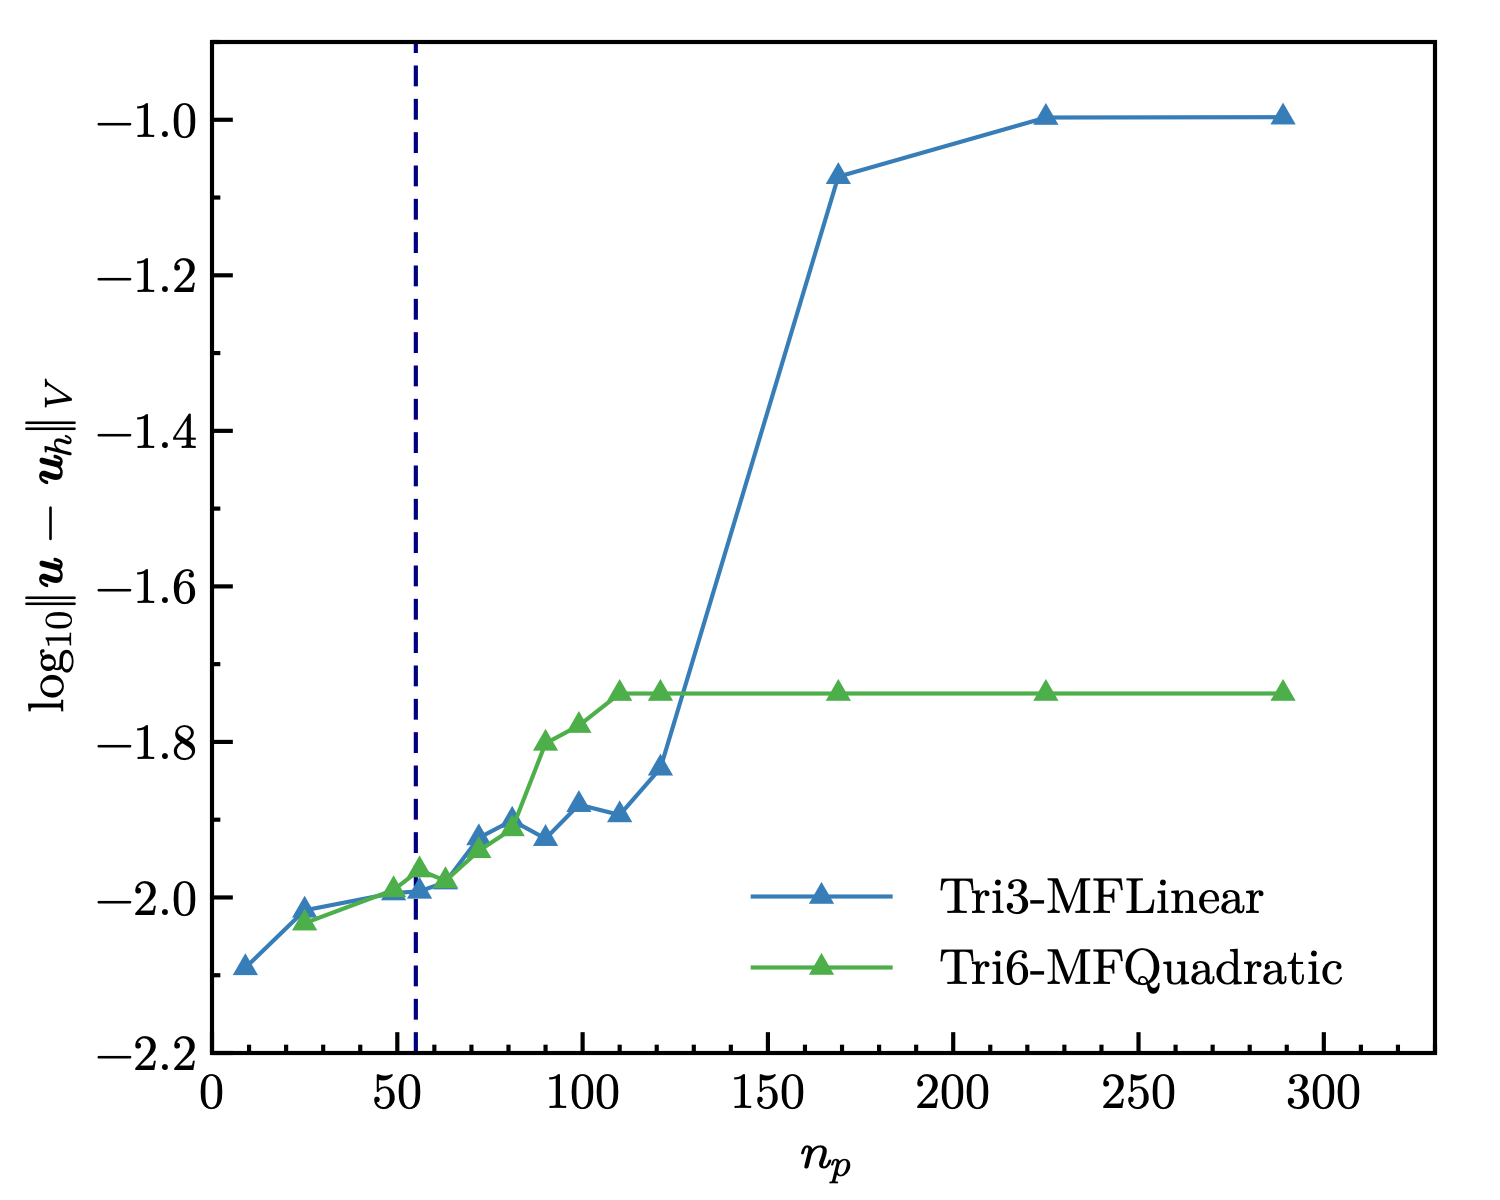
\includegraphics[width=0.45\textwidth]{figures/ch_4/plate_with_hole_4_L2_u.png}
    \phantomcaption\label{hole_32_L2_u}
    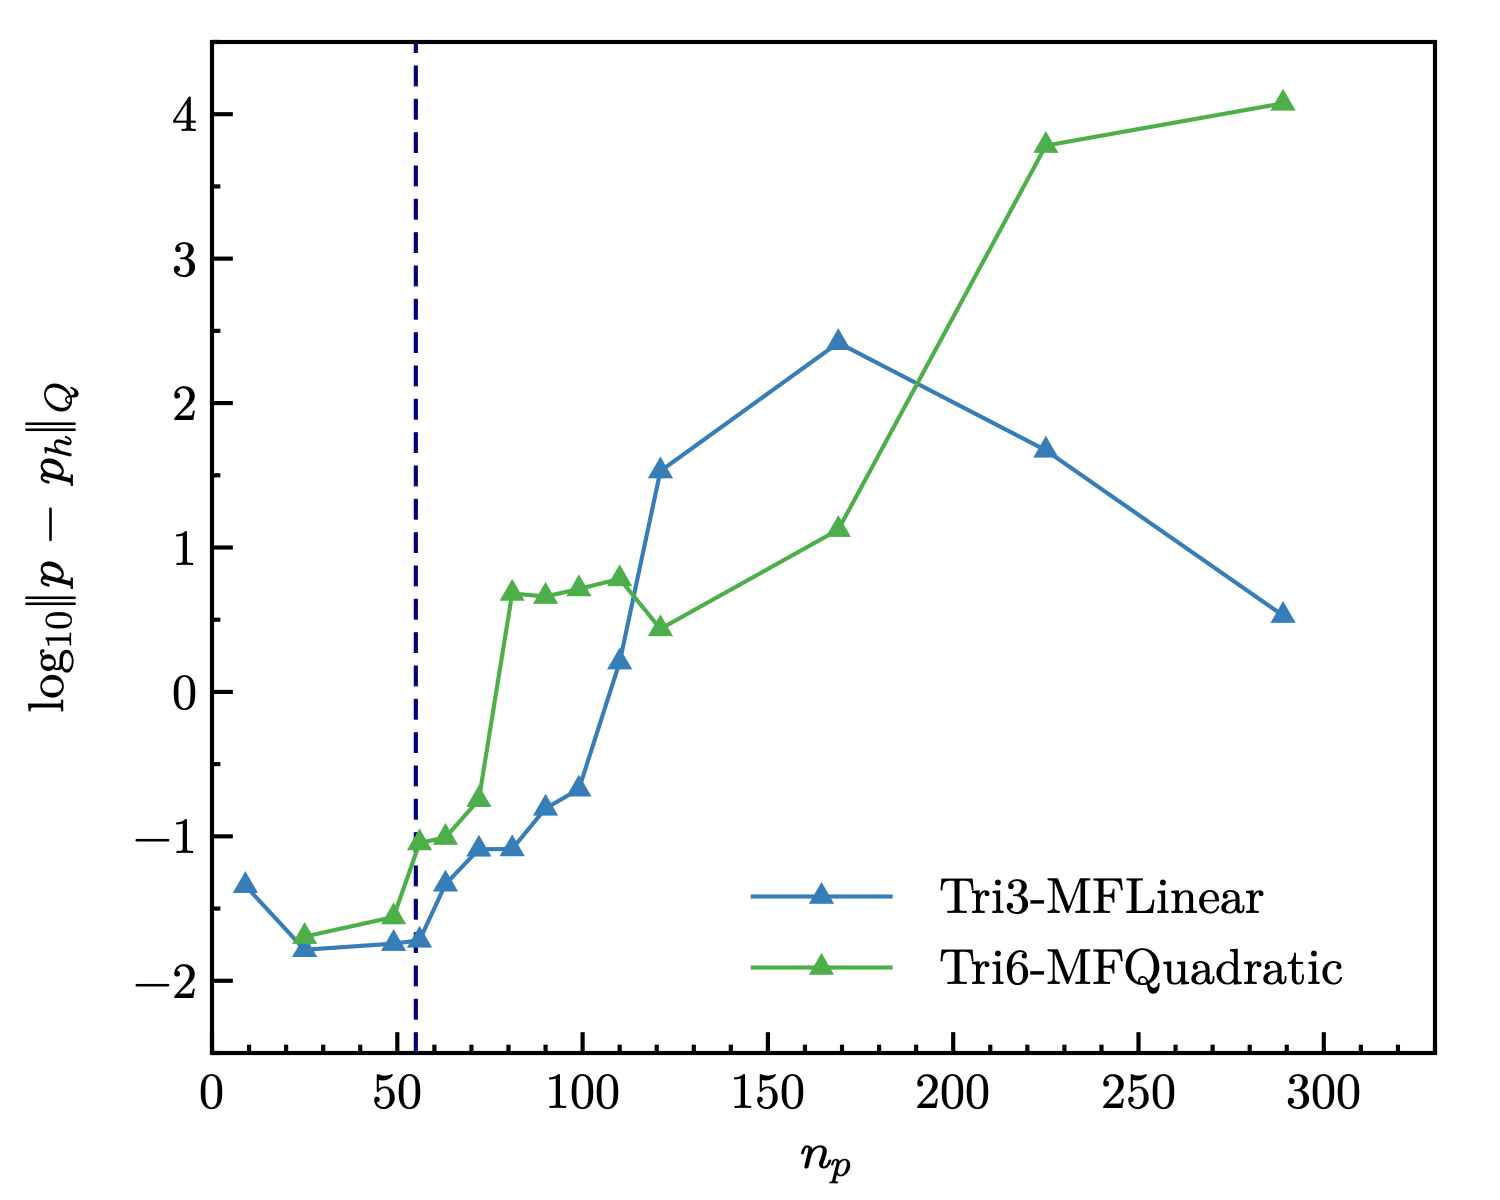
\includegraphics[width=0.45\textwidth]{figures/ch_4/plate_with_hole_4_L2_p.png}
    \phantomcaption\label{hole_32_L2_p}
    \end{subcaptiongroup}
\caption{\centering{悬臂梁问题$L2$误差与压力节点数量的关系:\protect\linebreak 
\subref{hole_4_L2_u}, \subref{hole_4_L2_p} $4\times 4$单元; 
\subref{hole_8_L2_u}, \subref{hole_8_L2_p} $8\times 8$单元;
\subref{hole_16_L2_u},\subref{hole_16_L2_p} $16\times 16$单元;
\subref{hole_32_L2_u},\subref{hole_32_L2_p} $32\times 32$单元;}}
\label{ch_4:fig:hole_l2}
\end{figure}

\subsection{Cook membrane 问题}
考虑经典的Cook membrane 问题,膜的尺寸如图\ref{ch_4:fig:cook}所示,右端沿着$y$轴正方向施加外部荷载$P=6.25$,膜的材料系数为杨氏模量$E=70$、泊松比$\nu=0.5-10^{-8}$。在这种情况下,$A$点的位移参考解为:$u_A=28$。
\begin{figure}[!h]
    \centering 
        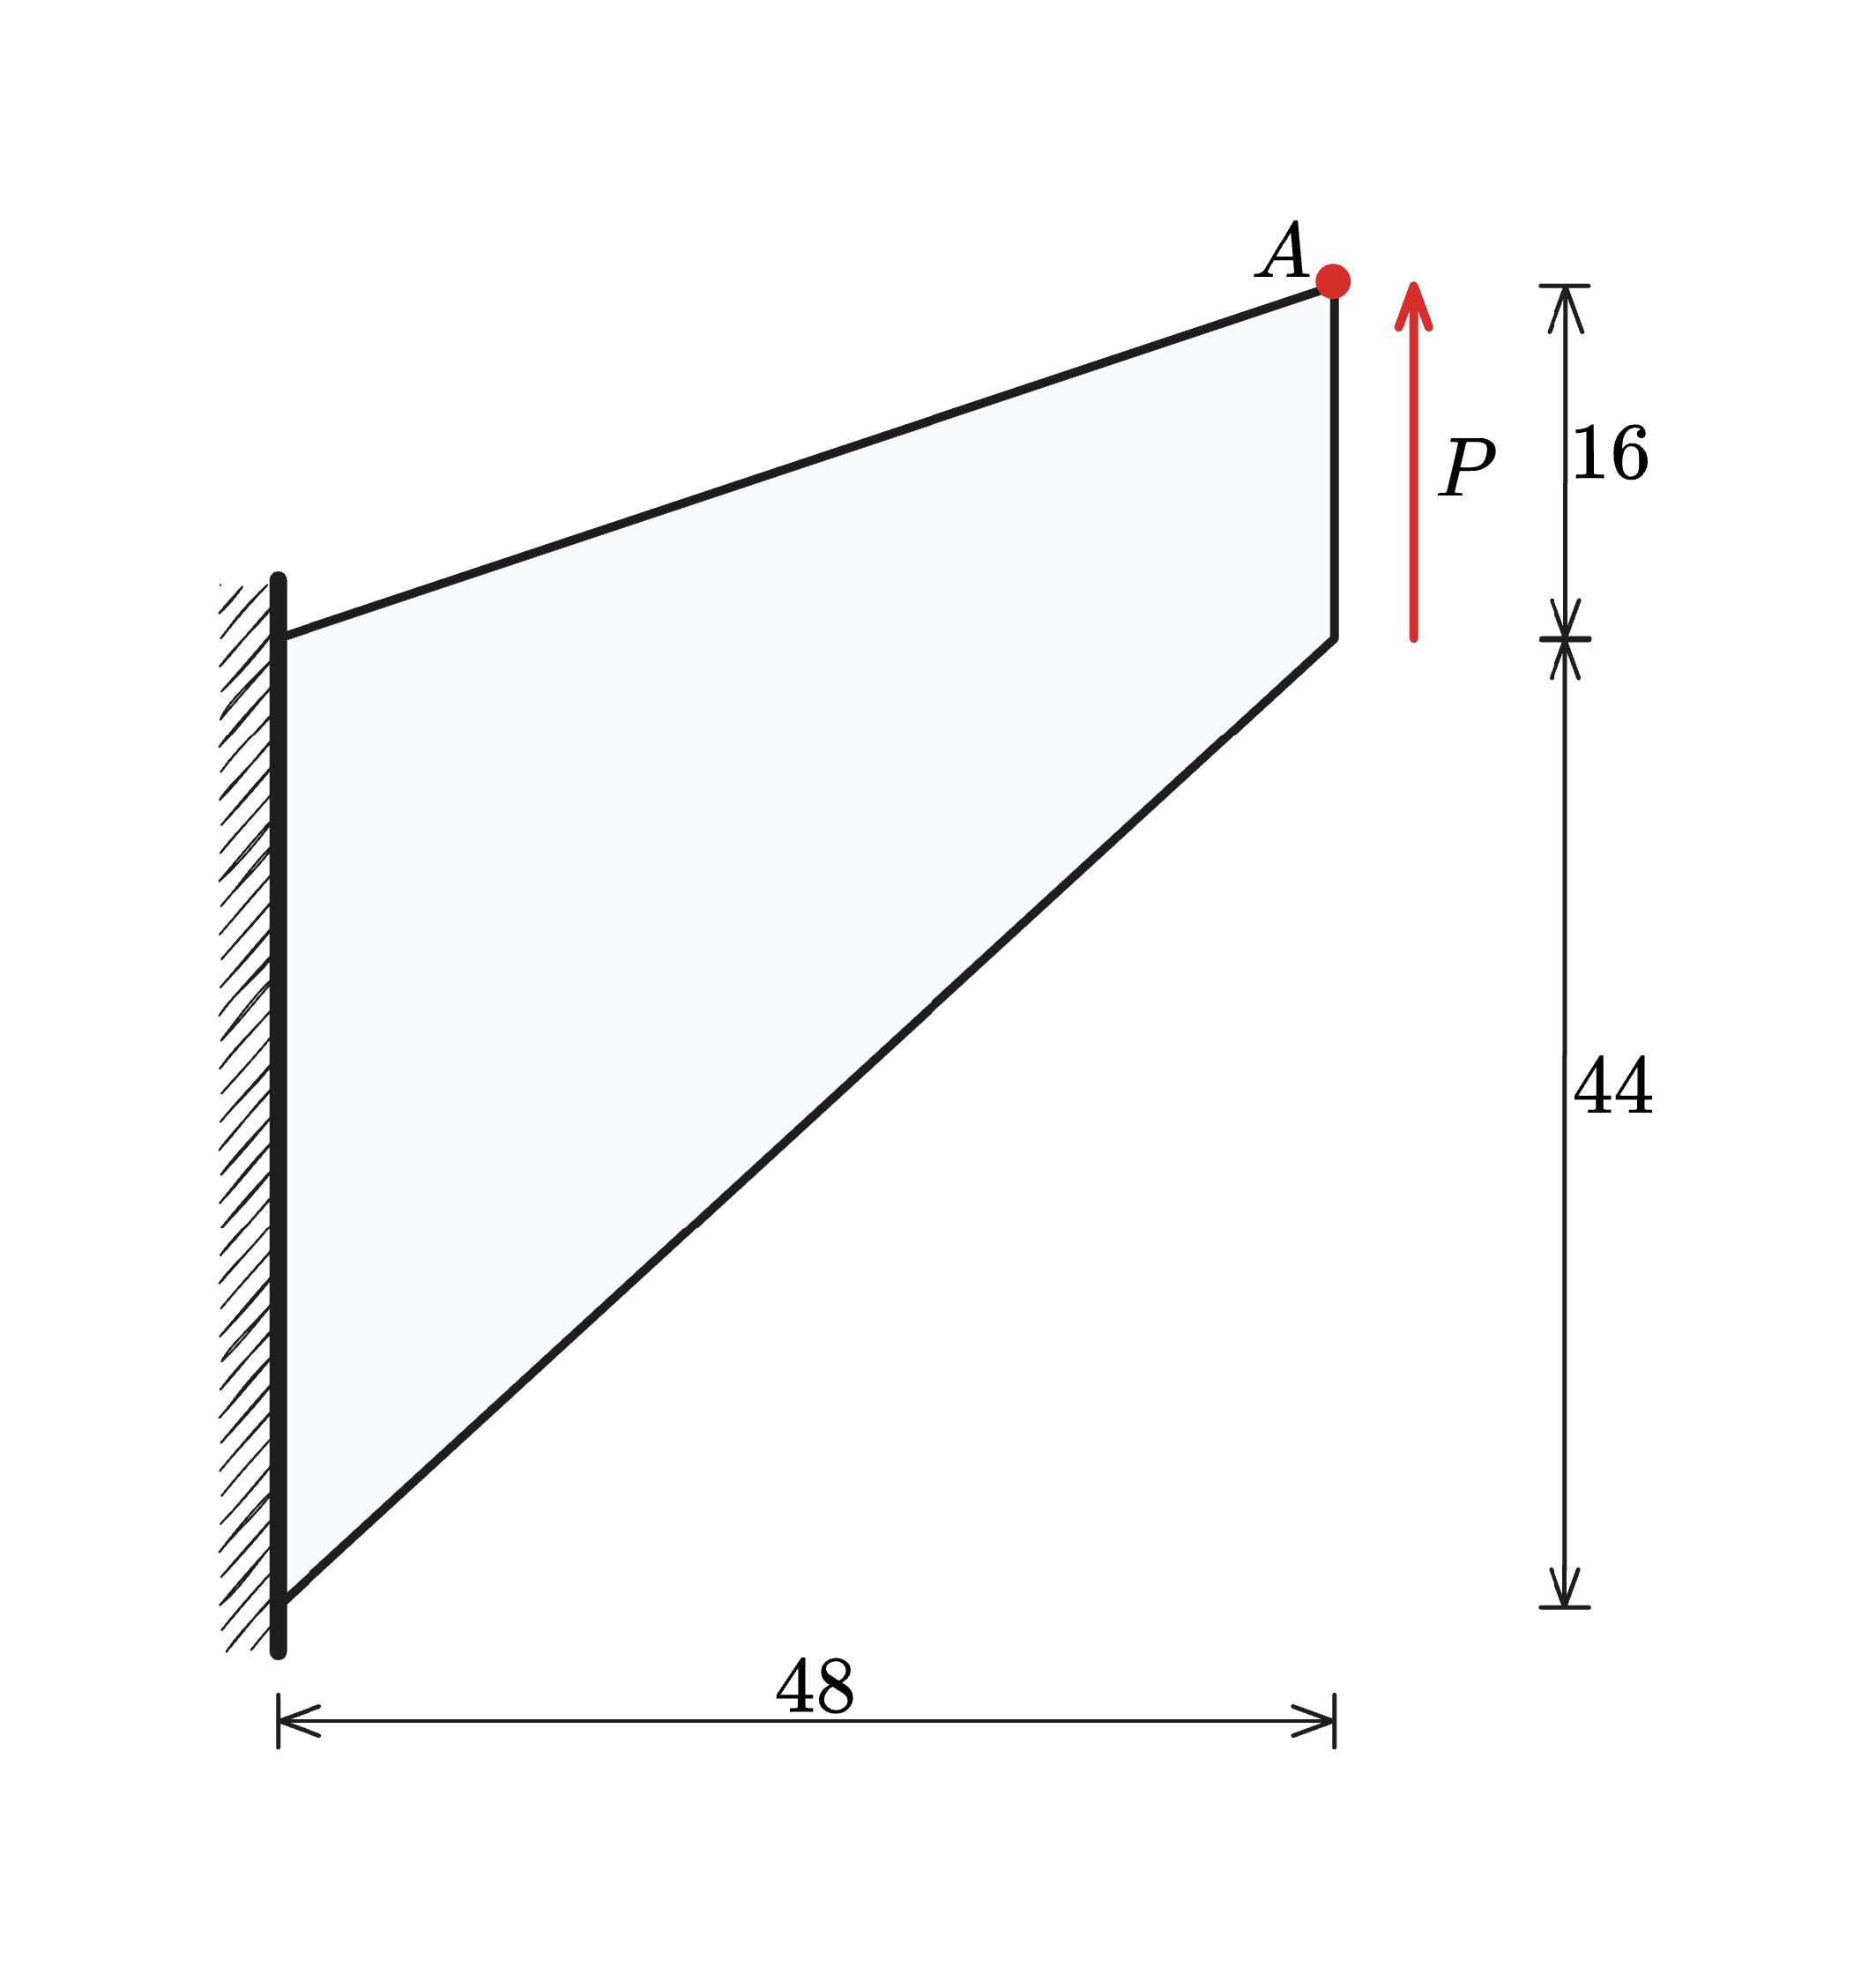
\includegraphics[scale=0.3]{figures/ch_4/cook.png}
        \caption{Cook membrane 问题模型}\label{ch_4:fig:cook}
\end{figure}

\section{小结}

本章建立有限元无网格混合离散方案,调整体积约束比为最优约束比以达到免体积自锁。首先对再生核无网格近似理论进行了系统讨论,详细说明了无网格形函数的构造过程,将混合公式中的压力采用无网格形函数进行离散,可任意调节压力节点的数量控制约束比。随后
